\section{Introduction}

Renewed international interest in lunar exploration, particularly through NASA's Artemis program and its international partners, has increased the need for reliable and accessible information about the lunar environment (NASA, 2020). The Moon has no protective atmosphere or global magnetic field, leaving its surface exposed to large temperature variations, radiation, micrometeorite impacts, electrostatic dust, and seismic activity. These hazards can affect crew safety and the operation of spacecraft and surface equipment. A range of scientific models already exists for studying individual lunar hazards. These models, however, are generally designed for specific hazards and operate as separate tools. Their outputs are difficult to combine into a single operational view or use together for forecasting. Mission planners may therefore need to consult several data sources and models when assessing environmental conditions, which complicates decision making. The Lunar Impact and Predictive Analysis System (LIPAS) was developed to address this fragmentation by bringing multiple lunar-hazard forecasts into a single decision-support platform. The system combines machine-learning predictions with physics-based models, public heliophysics data1, and adaptive weighting between the two approaches. The literature reviewed here describes specialized lunar hazard models and archives, while LIPAS explores how these sources can be combined with machine learning in a unified decision-support framework.

This study addresses three research questions:

RQ1: Can a hybrid lunar-forecasting system be developed by effectively combining machine-learning and physics-based approaches? RQ2: Can integrating multiple lunar environmental hazards and data sources into a unified forecasting and decision-support system improve operational usability? RQ3: Does the locked LIPAS hybrid improve prediction performance for selected lunar hazards relative to selected replicated public baselines and physics-only references? 1Heliophysics studies the Sun, the solar wind, and their interaction with planetary environments throughout the heliosphere.

\section{Overview of current models}

\subsection{General overview}

The study of lunar environmental conditions has historically relied on single-purpose models, each focused on a particular hazard. Although these models incorporate advanced scientific understanding in their respective domains, they remain limited when applied to operational mission planning because they do not provide integrated insights or unified predictive support. Each model was built to solve a specific scientific problem rather than to operate as part of a broader forecasting system. This creates a gap because the interactions among hazards cannot readily be analyzed.

\subsection{NASA DONKI model}

The NASA Database of Notifications, Knowledge, Information (DONKI) API provides near-real-time monitoring of solar flares, coronal mass ejections (CMEs), and solar energetic particle (SEP) events (NASA, 2023b). DONKI is valuable as a space-weather event catalog for radiation context, but it is event-driven and primarily reactive, with limited temporal coverage and incomplete data for continuous mission planning. It does not itself produce multi-day forecasts or integrate other hazard types, making it insufficient as a stand-alone planning tool.

\subsection{Temperature models}

Temperature predictions rely heavily on the Diviner Lunar Radiometer Experiment (Paige et al., 2010; Williams et al., 2017; NASA, 2023a), which provides detailed infrared measurements of surface temperature across the Moon. These measurements accurately characterize lunar thermal conditions, including uneven terrain, but do not themselves produce short-term forecasts. Apollo-era heat-flow measurements are similarly sparse and lack the temporal resolution required for short-term forecasting (Langseth et al., 1972). Neither source was designed to predict future temperature; both principally describe measured or reconstructed conditions. The early prototype used a simplified Diviner-style dayside surface-temperature relation, T = 392 cos0.25(z) -273, (1) where T is surface temperature in degrees Celsius and z is the solar zenith angle at the target coordinates. Legacy nightside profiles use polynomial fits derived from Apollo heat-flow measurements. Although deterministic, these stand-alone relations do not dynamically adjust to changing space-weather conditions.

\subsection{Lunar dust models (LADEE/LDEX)}

The lunar dust environment has been studied by the Lunar Atmosphere and Dust Environment Explorer's Lunar Dust Experiment (LADEE/LDEX), which documented dust-particle density and electrostatic activity (Horanyi et al., 2015; NASA Planetary Data System, 2015). LDEX is important for understanding surface hazards, but its data are limited to the LADEE mission epoch and orbital coverage, providing neither continuous global monitoring nor direct predictive capability. The mission ended in 2014, leaving substantial temporal and spatial gaps.

\subsection{Moonquakes and Apollo PSE}

Moonquake monitoring relies on the Apollo Passive Seismic Experiment (PSE) catalog. Recent reanalysis identified thousands of previously undetected moonquakes (Onodera, 2024). The PSE dataset is retrospective, cannot provide real-time forecasting, and does not integrate other hazards. Nevertheless, it contains statistical patterns tied to the lunar tidal cycle. LIPAS uses these patterns as physics/catalog context for moonquakerate estimates. Because deep moonquakes occur in clusters correlated with tidal stress between Earth and the Moon, recurring catalog patterns can be projected forward statistically even without real-time seismic sensors (Kawamura et al., 2017; Lammlein, 1977; Nakamura, 2005; Nunn et al., 2020).

\subsection{Micrometeorite prediction with MEM 3}

NASA's Meteoroid Engineering Model (MEM 3) estimates meteoroid collision rates (Moorhead et al., 2020). It is precise within its engineering domain but does not directly incorporate secondary operational effects such as dust lofting or the interactions of meteor-shower timing with surface operations. LIPAS therefore applies shower-calendar modulation and dust coupling to the MEM 3 baseline used in its physics path (American Meteor Society, 2026; International Meteor Organization, 2026; Szalay and Horanyi, 2015).

\subsection{GOES-18 radiation context}

NOAA's Geostationary Operational Environmental Satellite~18 (GOES-18) continuously monitors solar X-ray flux and

energetic-particle counts (National Oceanic and Atmospheric Administration, 2023). GOES measurements are made in Earth orbit and must be adapted for lunar-surface conditions because the Moon lacks a global magnetosphere. GOES-18 does not provide a dedicated multi-day lunar radiation forecast and was not designed specifically for lunar missions.

\subsection{Summary}

Individual models and archives such as DONKI, Diviner, MEM 3, PSE, and LDEX are essential for scientific research, but their limitations in coverage, integration, and predictive usability motivate a unified system. LIPAS combines the strengths of these single-purpose approaches with real-time NASA and NOAA space-weather data, historical lunar measurements, and a hybrid machine-learning architecture. The resulting framework is proactive and integrative, providing a comprehensive interface for mission planning and safety assessment while retaining the limitations of its source data and models.

\section{System overview: LIPAS}

\subsection{Prototype limitations and migration to a backend}

The original LIPAS prototype was a browser-based application in which data processing and machine learning were performed on the client side. As it grew, forecasts for physically constrained hazards such as temperature varied between training runs. This showed the need to retain stronger physical relationships and move processing to a backend that could support a more stable data and forecasting service. The application was therefore re-engineered as a server-assisted hybrid model with a Python backend. Data filtering, API polling, model training, and inference are handled on the server, which supplies a stable data service to the front-end dashboard. The current system can assign different levels of influence to machine learning and physics according to the hazard and current conditions.

\subsection{Hybrid forecasting and uncertainty architecture}

The core forecasting model uses an 18-feature input representation that contains hazard-related, temporal, spatial, and space-weather variables. Rather than processing only current conditions, the model receives a 72-step temporal window. It produces six target outputs: solar activity, radiation, temperature, moonquake rate, micrometeorite flux, and dust density. The larger input representation allows information from one environmental channel to contribute to the prediction of another. The temporal trunk is based on a long short-term memory architecture (Hochreiter and Schmidhuber, 1997). A physics-estimation function first calculates a physically grounded value for each hazard. A subsequent refinement step combines that value with the neural-network output, allowing machine learning to provide a correction instead of learning the complete physical relationship. For hazard channel i, the resulting prediction is bYhybrid,i = wibYML,i + (1 -wi)bYphysics,i. (2) The weight is evaluated from the current space-weather regime and the neural network's uncertainty: wi = max{0, min[1, (wbase,i + $\Delta$regime,i) × max(0.35, 1 -1.6$\sigma$ML,i S i )]}. (3) Here wbase,i is the baseline machine-learning weight, $\Delta$regime,i is an adjustment for the current storm posture, $\sigma$ML,i is the neural uncertainty estimate, and S i is the physical operating span of the channel. Uncertainty is estimated with Monte Carlo dropout: the network is evaluated repeatedly while a randomly selected subset of neural connections is disabled on each pass. Closely grouped outputs indicate a stable learned prediction, whereas a wider spread indicates greater uncertainty in the learned model.2 When $\sigma$ML,i rises, Eq. (3) reduces the neural contribution and shifts the forecast toward the physics baseline. Where physics provides a strong basis, LIPAS assigns greater weight to the physics path. In the locked production blend, temperature, moonquakes, micrometeorite flux, and dust are predominantly physics-led, while solar activity and radiation retain larger machine-learning weights. The backend also supports optional ensemble forecasts for uncertainty estimation, although the evaluated production path uses a single locked temporal model.

\subsection{Development of the hybrid framework}

The current LIPAS implementation uses HTML, CSS, and JavaScript for the front end and a Python/TensorFlow backend for data ingestion, model training, physics blending, and forecast serving (Google TensorFlow Team, 2026; Chollet et al., 2015). Multiple production training runs were completed. The reported quantitative evaluation used the second training-run model because it was the best-performing completed production model when the model was locked for testing. Its chronological held-out test RMSE was approximately 4.97, compared with approximately 13.66 for the corresponding persistence baseline; no later completed run had surpassed it at the evaluation cutoff. Earlier prototype experiments used the browser-based neural network that preceded the Python hybrid backend. They are treated as developmental diagnostics rather than evidence of current model performance because they lacked the architecture and baseline framework used in the reported evaluation. The locked production model was subsequently evaluated using the framework in Section 4.

\subsection{Data ingestion and pipeline orchestration}

The backend handles real-time data streams through a modular ingestion pipeline that queries, cleans, and normalizes external APIs into the 18-feature representation. The pipeline joins CME events from DONKI, solar indices from the NOAA Space Weather Prediction Center, and interplanetary magnetic-field data from OMNI (NASA, 2023b; National Oceanic and Atmospheric Administration, 2023; NASA Goddard Space Flight Center, 2026; King and Papitashvili, 2005). These space-weather feeds are combined with LRO Diviner thermal maps, CRaTER radiation logs, and LADEE/LDEX dust measurements (NASA, 2023a,c; NASA Planetary Data System, 2015). Long-term baselines include Apollo PSE data, Apollo heat-flow measurements, MEM 3, and peer-reviewed micrometeorite-flux data. 2This is the uncertainty that comes from the model, or from gaps in the training data. LIPAS is a hybrid forecasting system in which machine learning is used only where it can improve on an established physics calculation. Where a physics relation already describes a hazard well, that relation remains the primary estimate, and the learned correction is downweighted or switched off (Section 3.2).

\begin{figure*}[t]
\centering
\begin{minipage}{0.48\textwidth}
\centering
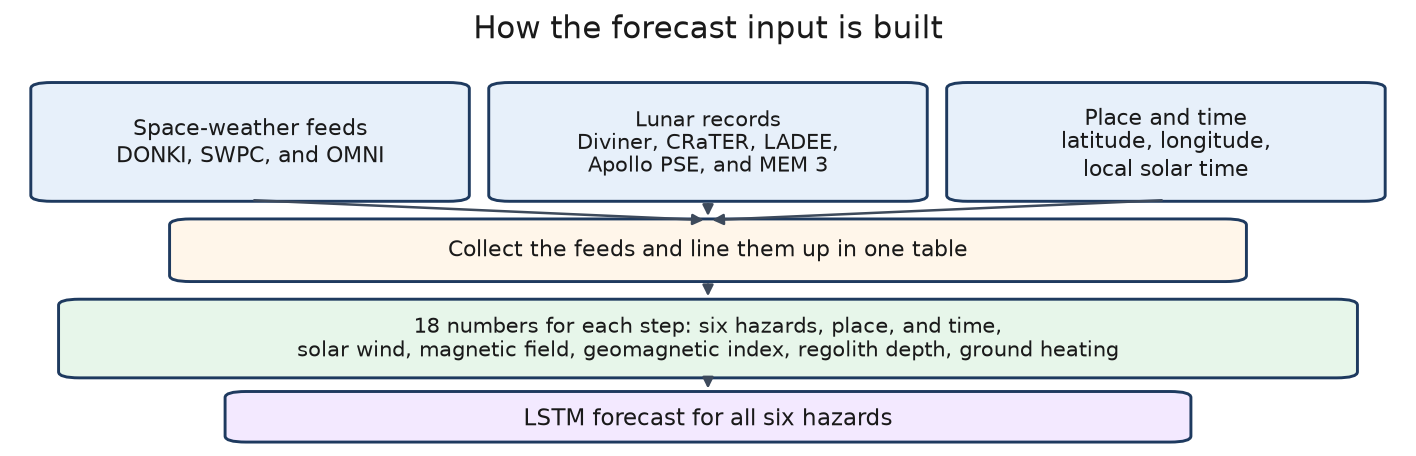
\includegraphics[width=\linewidth]{figures/fig_architecture_data_path.png}
\end{minipage}\hfill
\begin{minipage}{0.48\textwidth}
\centering
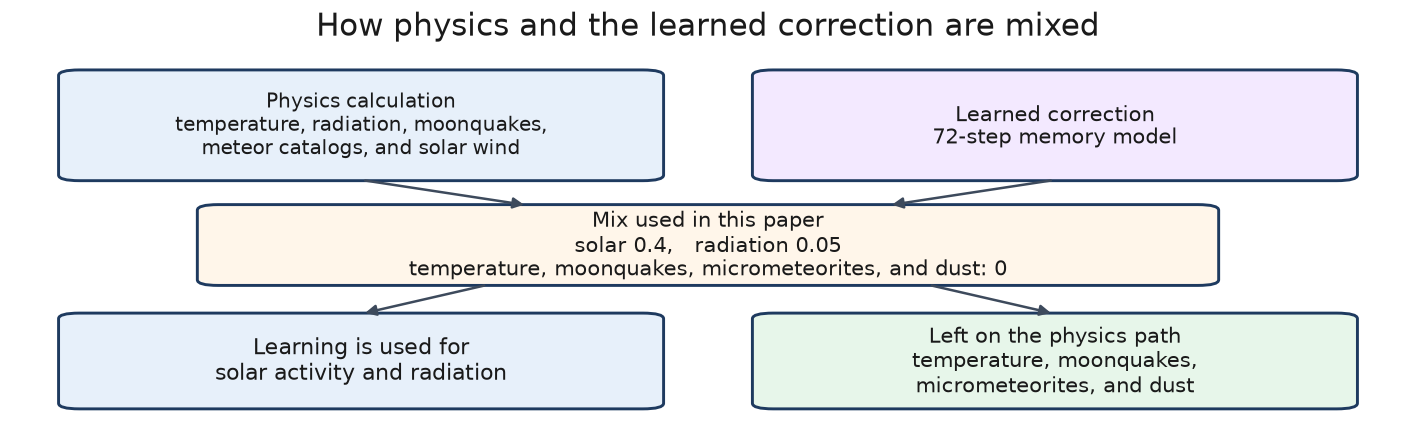
\includegraphics[width=\linewidth]{figures/fig_architecture_blend.png}
\end{minipage}
\caption{How data reach the forecast, and how physics and the learned correction are mixed. (a) Data path. (b) Locked mix: solar activity weight 0.4 and radiation 0.05; the other four hazards stay on the physics calculation.}
\label{fig:arch}
\end{figure*}

\subsection{Commandcenter dashboard and map visualization}

The user interface was overhauled after the prototype limitations were identified. The resulting mission-control-style interface uses CSS Grid and Flexbox and consists of a dashboard, mission planner, and Cesium globe (Cesium GS, 2026; Chart.js Contributors, 2026). The dashboard includes more than 50 named lunar locations and a coordinate search interface for arbitrary sites. It provides topographic maps with hazard overlays, 30day outlooks, particle-flux visualizations, and warnings and recommendations for mission planning. Historical and predicted trends can be displayed as line, bar, or area charts. The missionplanning interface accepts mission parameters and duration targets. Based on available forecasts, it proposes EVA departure windows, assesses landingzone conditions, and generates an exportable mission plan. A Luna Assistant provides additional hazard information. These dashboard and planning views are the operator-facing surface of LIPAS. The Cesium page supplies an interactive two or threedimensional lunar map with time-dependent overlays for dust, radiation, and solar drivers. Together these views form the redesigned LIPAS operator interface used after the prototype migration. \begin{figure*}[t]
\centering
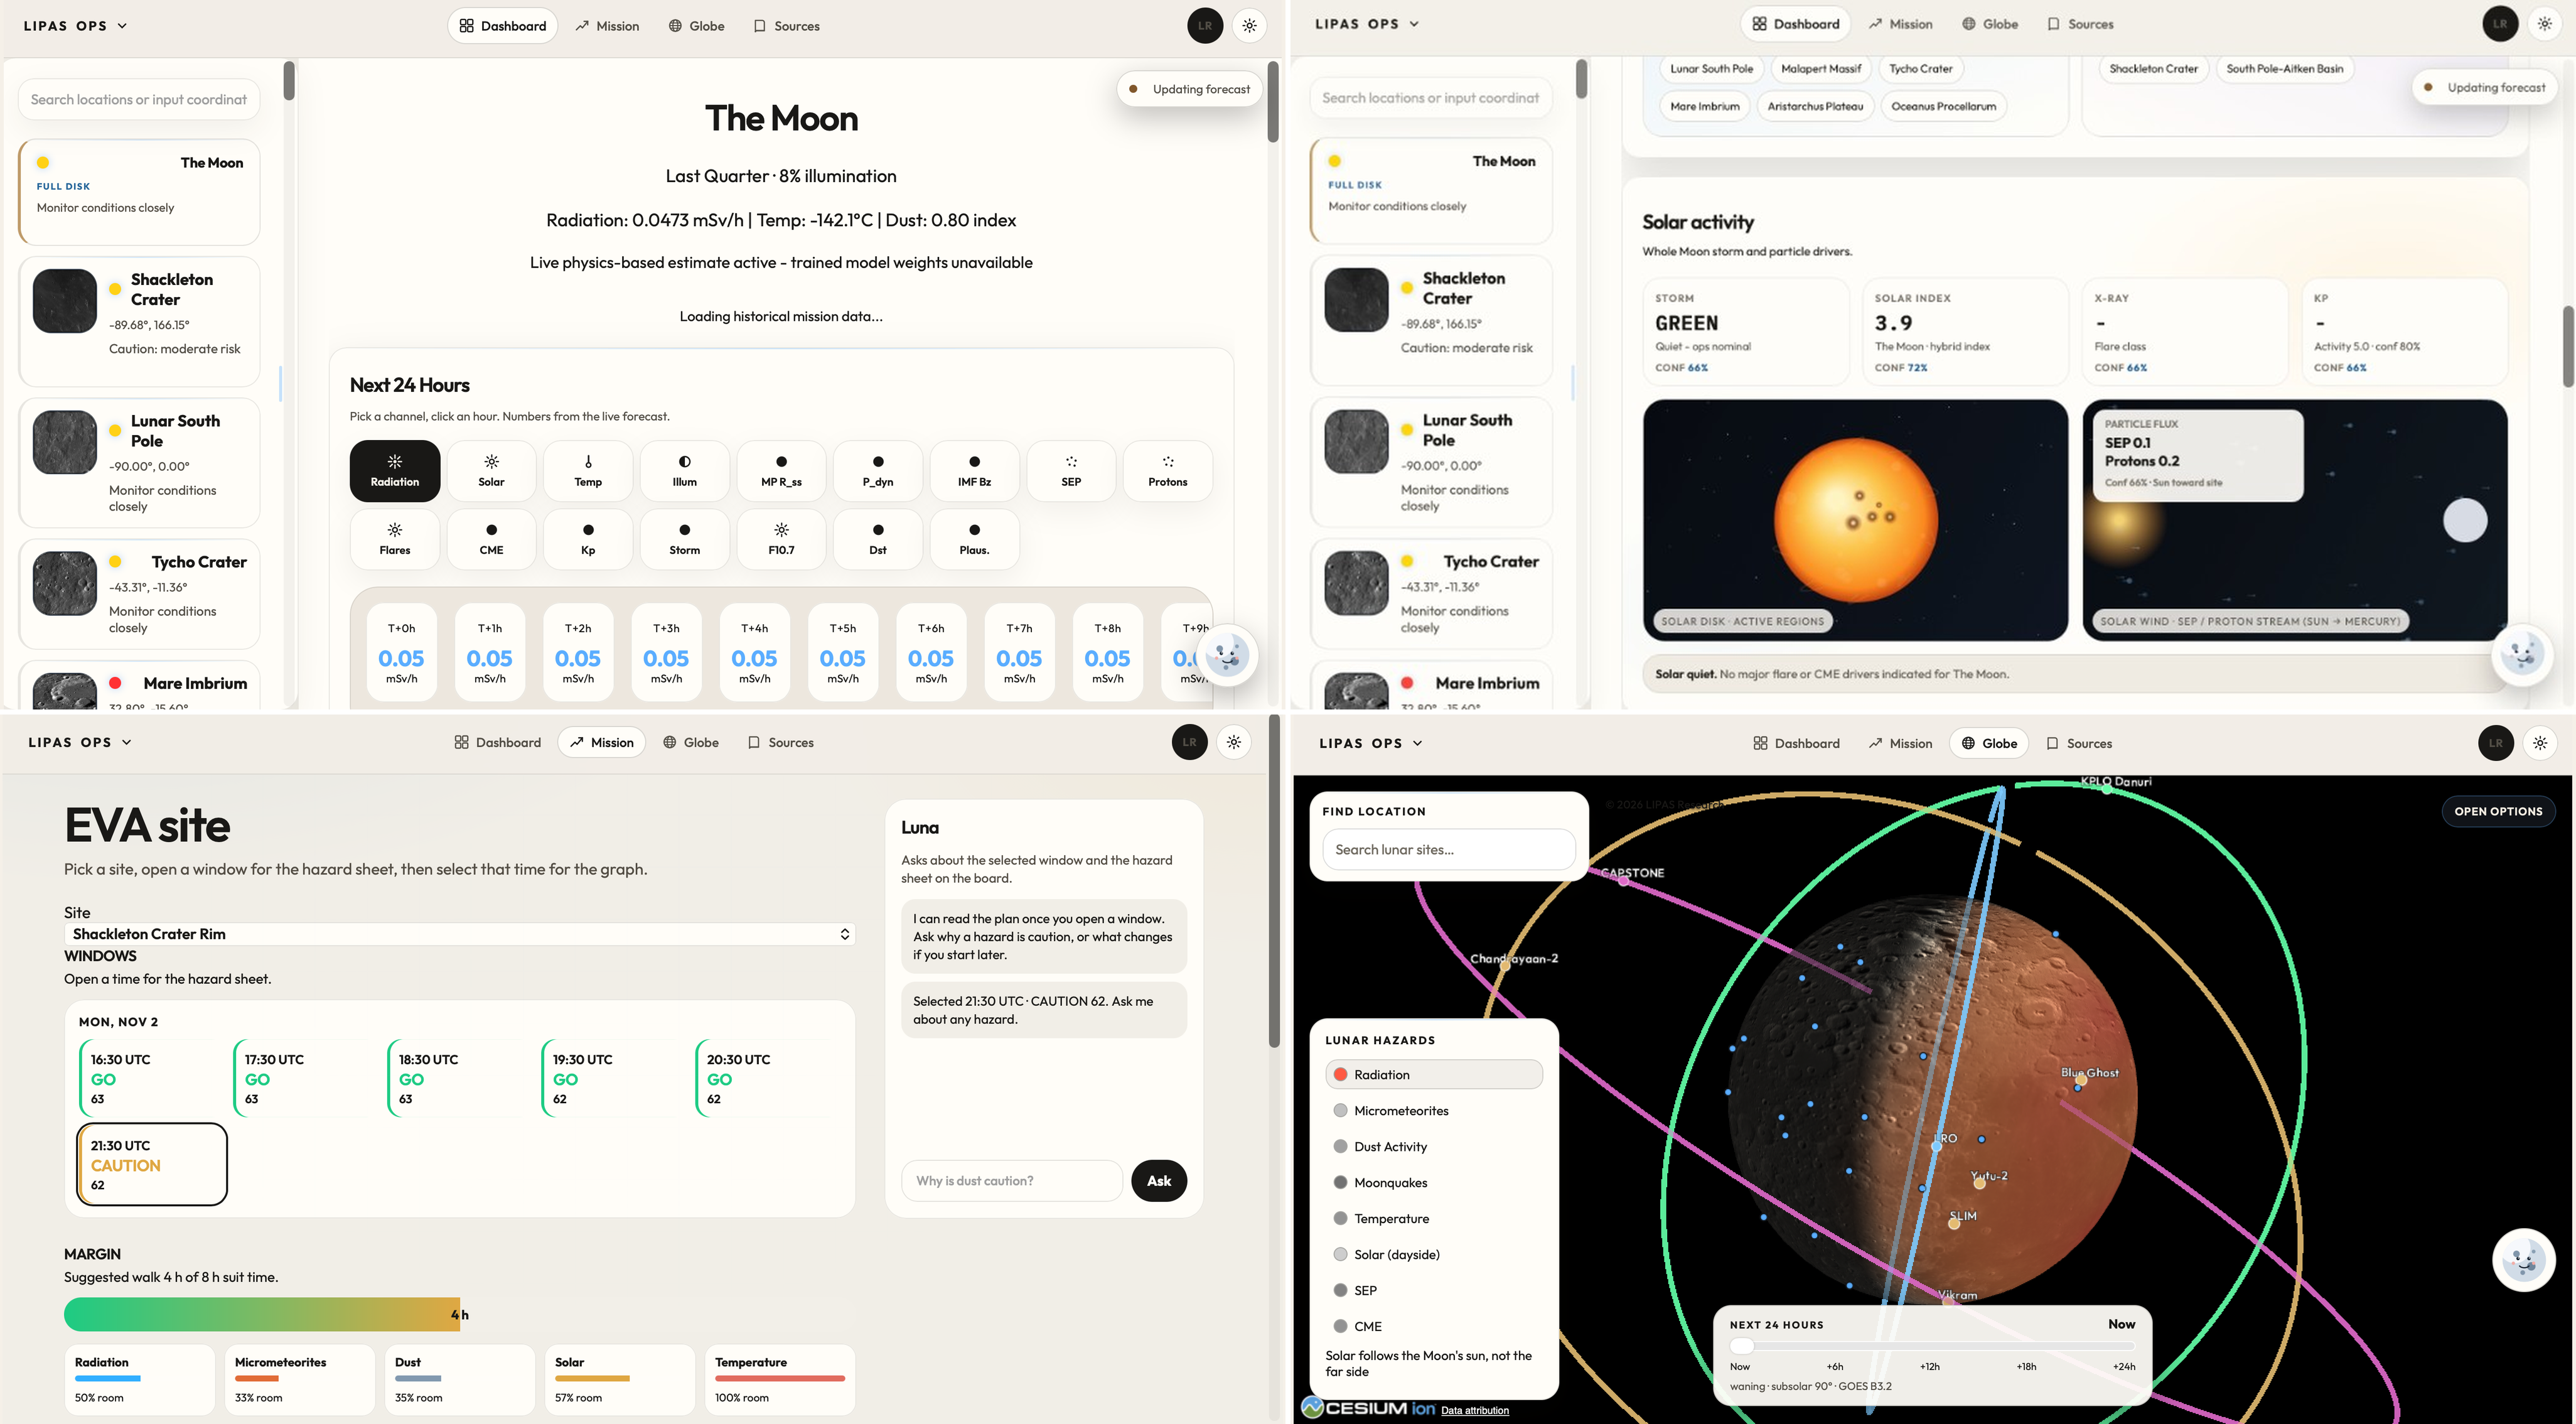
\includegraphics[width=\textwidth]{figures/fig_operator_workflow_four_panel.png}
\caption{Representative LIPAS operator workflow (dashboard, solar activity, mission planner, and globe views).}
\label{fig:workflow}
\end{figure*}

Figure~\ref{fig:workflow} shows the operator interface in four panels: site selection, diagnostics, exportable mission reporting, and the Cesium globe. All quantitative window, mission, and ablation scores in this paper use the locked production model; the April prototype diagnostic remains separate.

Panels: (a) site selection and hazard map; (b) forecast drivers and diagnostics; (c) exportable mission report; (d) Cesium globe. Dashboard: \url{https://lipas.netlify.app}

\section{Methods}

\subsection{Experimental design and evaluation framework}

The research was divided into three phases, each addressing one research question. The first focused on developing LIPAS and identifying lessons from that process, including the April prototype diagnostic. The second examined operational use in a simulated mission. The third evaluated whether the locked hybrid system improved predictive performance relative to established physics-based and agencystyle reference approaches. All reported quantitative evaluations in Windows A and B, the mission simulation, and the ablation used the locked production model from the second training run. The April prototype scores are separate and are not pooled with those locked-model results.

\subsubsection{Phase 1: development of the hybrid model}

The first phase examined the transition from the browser prototype to the hybrid system. It included a daytime prototype evaluation at 0$^\circ$N, 0$^\circ$E from 5 to 19 April 2026. The purpose was not to establish operational accuracy, but to identify weaknesses in the client-side machine-learning approach and determine which channels required a physics-based foundation. Treating all six hazards as machine-learning problems produced unstable results for strongly physicsconstrained hazards. Consequently, temperature, moonquakes, dust, and micrometeorites were kept predominantly physics-based, while machine learning was given a larger role in solar activity and radiation. This phase also established the 18feature input structure (hazard, time, place, and space-weather numbers), the 72step temporal window, the physics\_estimate paths (Sections 3.2 and 4.4), and adaptive hybrid weighting (Eqs. 23). These components were combined into the locked model used in the remaining phases. Continuous colocated measurements are unavailable for all six hazards, so comparison targets are called evaluation labels rather than ground truth unless a direct observation exists (Table 1). Performance used RMSE and MAE. Site geometry for Windows A and B is shown in Figure 3. Predictions in the locked windows were compared with persistence, physicsonly references, and replicated public baselines (Section 4.4), replayed from archived OMNI, NOAA, GOES, and DONKI data.

\subsection{Qualitative comparison criteria}

Before the quantitative windows, LIPAS and selected agency models and archives are scored on nine ordered criteria. Labels run from None to Very High and are not converted into a numeric total or summed rank. Appendix B records the scoring rules; Table 2 summarizes the matrix. The locked-model RMSE and MAE studies remain the primary quantitative evidence for research question 3. Hazard coverage. None: no hazard addressed; Very Low: one hazard; Low: up to two hazards; Moderate: three to four hazards; High: five hazards; Very High: six or more integrated hazards. Datafusion capability. None: one dataset; Low: multiple datasets without integration; Moderate: partial integration; High: integrated multisource system; Very High: real-time dynamic multisource fusion. Temporal forecasting ability. None: archival only; Low: event-driven alerts without a time horizon; Moderate: short-range estimates for a narrow domain; High: multi-day forecasting for one or more hazards; Very High: multi-day forecasting across all hazards. Spatial coverage. None: no spatial resolution; Very Low: specific historical sites; Low: one region or polar area; Moderate: broad regional coverage; High: global or near-global coverage; Very High: complete lunarsurface coverage with location selection.

\subsubsection{Phase 2: operational mission evaluation}

The second phase examined whether integrating several environmental hazards could support operational usability during a simulated lunar mission. A controlled radiation-focused EVA scenario used a timeline of 7 h 37 min, matching the duration of the second Apollo 17 EVA. LIPAS was monitored at fixed intervals and compared with information an operator would receive from separate public NASA and NOAA products, including GOES, NOAA SWPC, and DONKI. The same predefined caution and no-go thresholds were applied to each pathway. The comparison focused on when each system produced warnings and when the simulated EVA reached caution or no-go conditions. It did not establish that LIPAS is safer than NASA systems or measure usability with mission personnel.

\subsubsection{Phase 3: quantitative prediction evaluation}

The third phase evaluated the locked hybrid system against physics-based and replicated NASA/NOAA reference approaches at three locations: 0$^\circ$N, 0$^\circ$E, Apollo 11, and Nobile Rim (Fig. 3). Window A covered 518 July 2026 (predominantly lunar night); Window B covered 22 July4 August 2026 (predominantly lunar day). For Window B micrometeorites, LIPAS used MEM 3 with American Meteor Society (AMS) showercalendar modulation, while the replicated comparison did not apply that AMS shower calendar. Results then report the studies in matching order: prototype diagnostics, qualitative comparison, fourteen-day windows, mission simulation, and input ablation.

\subsection{Qualitative comparison criteria (continued)}

Realtime operational capability. None: historical only; Low: archival access with significant delay; Moderate: nearreal-time with limited updates; High: live feeds with regular updates; Very High: continuous real-time data with automated processing. Robustness and stability. Low: limited coverage or known gaps; Moderate: functional with notable external dependencies; High: wellvalidated and stable in a narrow domain; Very High: continuously calibrated missiongrade instrumentation with a long operational history. Validation strength. None: no comparison; Low: informal or limited comparison; Moderate: structured comparison over a limited period; High: peerreviewed validation against direct measurements; Very High: direct physical measurement, selfvalidating by design. Usability and operational readiness. Very Low: raw scientific data requiring specialist processing; Low: technical interfaces; Moderate: accessible API or web portal; High: clear operational interface; Very High: interactive dashboard for nonspecialist mission planners. Openness and accessibility. Low: restricted or proprietary; Moderate: archives requiring registration or processing; High: open API or published datasets; Very High: fully open browser-based access without setup. No aggregate result in this paper represents validation against simultaneous in-situ measurements of all six hazards across the lunar surface. An ablation analysis later replaces selected inputs with Window A means while holding the locked model fixed (no retraining). Baseline configurations and hazard-specific replication continue in Sections 4.34.4.

Figure 3: Lunar locations used in the reported studies: the equatorial reference, Apollo 11, and Nobile Rim. Performance was evaluated primarily by root mean square error (RMSE) and mean absolute error (MAE): The Window B micrometeorite comparison used the MEM 3 seasonal background with American Meteor Society (AMS) shower modulation for LIPAS, while the replicated comparison omitted that additional shower term. This tests the effect of explicitly representing shower timing during the Perseid period, not general superiority over NASA's complete meteoroidmodeling framework. An ablation analysis removed selected inputs while holding the remaining conditions fixed. Conditions included the full hybrid model, removal of solar/storm drivers for radiation, removal of micrometeorite context for dust, an MLonly path, and a physicsonly path. Resulting predictions were compared with the

\subsection{Baseline configurations and control environments}

Reference predictions were obtained from public databases, peerreviewed formulas, engineeringmodel exports, and agency documentation. In this paper, a replicated NASA/NOAA reference means an authorimplemented reconstruction from those public materials; it does not mean that internal, proprietary, operational, or flight-certified agency software was executed. MEM 3 is treated separately because the comparison used an engineeringmodel export available to the project. Where an established product did not provide a direct multi-day lunar prediction for a study interval, the relevant public method was reproduced as closely as the documented equations and open data allowed. For every hazard, the study recorded the source, procedure, and whether the target was a direct measurement, engineering baseline, or physics proxy. In the mission simulation and ablation tests, coordinates and physical constants were held fixed while selected inputs were altered. The mission scenario used archived quiet conditions as a background and injected controlled changes, with status checked at fixed intervals. The ablation tests replaced selected driver or hazard inputs with their Window A means as sensitivity tests. Table 1 (next) summarizes provenance for each evaluation target. Section 4.4 then specifies how each hazard baseline was replicated for Windows A and B, including the physics\_estimate paths used when a public product did not already publish a multi-day lunar forecast for the study coordinates and dates. Where a channel mixes an engineering export with an authoradded term (for example MEM 3 plus the AMS shower calendar), both pieces are stated explicitly so that a reader can replay the comparison without assuming access to internal agency software. Persistence and physicsonly references share the same replay calendar and site list as the locked hybrid forecasts. Control environments therefore differ by which drivers are visible to each pathway, not by which dates or coordinates are evaluated. That separation is what lets the later Results tables attribute RMSE and MAE changes to the locked blend, the AMS term, or an ablated input rather than to a silent change of study geometry. full system using RMSE and MAE.

Table 1: Provenance and interpretation of the six quantitative evaluation targets. Channel Principal target construction What is directly observed Validation status Solar activity Archived OMNI/SWPC indices and DONKI event context mapped to the study's solar-activity label Solar-wind, field, flare, and geomagnetic drivers Constructed label from measured drivers Radiation CRaTER-calibrated background combined with archived solar and proton-event terms Orbital particle and space-weather measurements Observation-constrained lunarsurface proxy Temperature Diviner/Apollo-constrained thermal equations evaluated at each site and time Orbital temperature maps and historical heat-flow measurements Observation-constrained physics proxy Moonquakes Apollo PSE catalog rates with tidal, terminator, and location adjustments Historical Apollo seismic events Historical-catalog proxy Micrometeorites MEM 3 engineering output with a separately stated AMS shower-timing term MEM 3 output and terrestrial shower timing Engineering-model/shower proxy Dust LDEX-informed background with impact, local-time, and terminator terms Historical orbital dust detections Observation-informed physics proxy

\subsection{Baseline replication and model specifications}

\subsubsection{Temperature}

Temperature baselines used lunar thermal physics constrained by Diviner observations and Apollo nightside measurements (Vasavada et al., 1999; Paige et al., 2010; Hayne et al., 2017; Williams et al., 2017; Langseth et al., 1972). On the dayside, surface temperature was computed from the Stefan-Boltzmann balance T = (1 -$\alpha$)I0 cos $\theta$ $\epsilon$$\sigma$ !1/4 , (6) where I0 is solar irradiance adjusted for Earth-Sun distance, $\alpha$ is surface albedo3, $\epsilon$ is emissivity, $\sigma$ is the Stefan-Boltzmann constant, and $\theta$ is the local solar-incidence angle. Nightside temperatures were calculated with an Apollo-based cooling curve and adjusted for latitude and a small interior heat term. Site reflectivity, emissivity, terrain, and thermal inertia were taken from the LIPAS site data. Where available, Diviner observations could further constrain the estimate. The early prototype also used Eq. (1); the reported studies used Eq. (6) and the Apollo-based nightside model. An equivalent form used in the implementation is (1 -$\alpha$)Is = $\epsilon$$\sigma$T 4. (7)

\subsubsection{Solar activity and radiation}

Solar and radiation baselines were built from public space-weather data rather than a direct lunar radiation forecast. Solar activity used OMNI2 and SWPC quantities including Kp, the 3Albedo is the fraction of incoming radiation reflected by a surface; emissivity describes how efficiently that surface emits thermal radiation. interplanetary magnetic-field component Bz4, solar-wind speed and density, and F10.7 where available. DONKI flare, CME, geomagnetic-storm, and SEP records were included for the study dates. The radiation path used a CRaTER-based galactic-cosmicray background of approximately 0.38 mSv day-1, converted to an hourly value and adjusted for solar activity (Spence et al., 2010; Schwadron et al., 2014; NASA, 2023c). Additional quiet, storm, and SEP terms used Kp, southward Bz, high solar-wind speed, GOES proton measurements, and solar activity. A small latitude adjustment was applied near the lunar poles. GOES X-ray and proton measurements were model inputs, not direct lunar-surface radiation measurements.

\subsubsection{Micrometeorites}

Micrometeorite baselines were replicated from the project's MEM 3 export (Moorhead et al., 2020). The annual flux set the principal background level, and available highand low-density ranges represented seasonal variation. LIPAS added AMS-based meteor-shower modulation separately from the basic MEM 3 baseline. A latitude term was applied only in the LIPAS physics path. For Window B, the replicated comparison used MEM

3 without the AMS shower term, while LIPAS used MEM 3

plus shower modulation. This directly isolates the effect of meteor-shower timing.

\subsubsection{Dust}

Dust baselines used LADEE/LDEX data rather than a live global forecast. The model combined a normal background with dust associated with micrometeorite impacts, enhanced dust near 4The interplanetary magnetic field is carried outward by the solar wind; a sustained southward Bz component can indicate stronger coupling with Earth's magnetic environment.

terminators [5], an optional LDEX local time factor, and a small regolith depth effect [6] (Colwell et al., 2007; Horanyi et al., 2015; Stubbs et al., 2006). It is therefore a physics proxy based on LDEX observations, not a claim of continuous dust measurement at the Artemis sites.

\subsubsection{Moonquakes}

Moonquake baselines used the Apollo PSE catalog. The model combined deep, shallow, and thermal moonquake rates, enhanced activity near terminators, a small equatorial preference for deep events, and a weak regolith effect. No real-time lunar seismometer network was assumed. The output is a catalog-based physics proxy rather than a direct measurement of current activity at the study sites. Persistence baselines assumed that the latest known value remained constant. Physicsonly references were generated from the common replay data. RMSE and MAE were calculated for LIPAS against persistence, physicsonly paths, and each replicated reference baseline. The mission simulation used common LIPAS outputs and baselines throughout the Apollo 17length timeline, and the ablation study used the same replay data while removing selected inputs or pathways. [5] The lunar terminator is the moving boundary between illuminated day and darkness, where rapid electrical and thermal changes may affect dust behavior. [6] Regolith is the loose layer of fragmented rock and dust covering the lunar surface.

\section{Results}

\subsection{Prototype diagnostics}

The preliminary studies evaluated the browser prototype under daytime conditions at 0 deg N, 0 deg E from 5 to 19 April 2026. One study tracked all six hazards against weakly replicated NASA and NOAA baselines. Another compared temperature with a Divinerstyle dayside relation. The aim was to see where the prototype failed under that weakreplica setup before the locked hybrid model was trained. \begin{figure}[t]
\centering
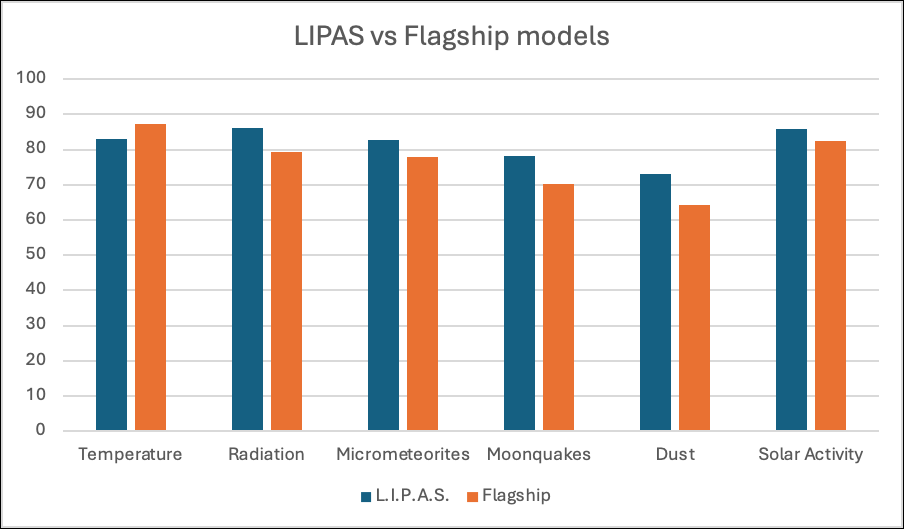
\includegraphics[width=\linewidth]{figures/fig_prototype_draft14.png}
\caption{Preliminary LIPAS versus replica scores across six hazards (5 to 19 April 2026, daytime, 0$^{\circ}$N 0$^{\circ}$E).}
\label{fig:proto}
\end{figure}

Figure~\ref{fig:proto} summarizes that April diagnostic across six hazards. It is not the fourteen-day evaluation in Section 5.3. Temperature is the only hazard where the replica scores higher; the prototype is higher on radiation, micrometeorites, moonquakes, dust, and solar activity. The temperature miss is the actionable finding that motivated the physics-led temperature path in the locked model. Figure 5 on the next page shows the same miss as a daytime temperature trace against a Divinerstyle dayside estimate. Section 5.2 then scores LIPAS against selected agency models and archives on the nine qualitative criteria defined in Section 4.2. Figure 4: Preliminary LIPAS versus replica across six hazards (5 to 19 April 2026, daytime, 0 deg N, 0 deg E). Prototype vs weak replicas per hazard (April diagnostic). replica scores

\subsubsection{April temperature trace}

The same April days, at 0$^\circ$N, 0$^\circ$E, are plotted below against a Divinerstyle dayside estimate. \begin{figure}[t]
\centering
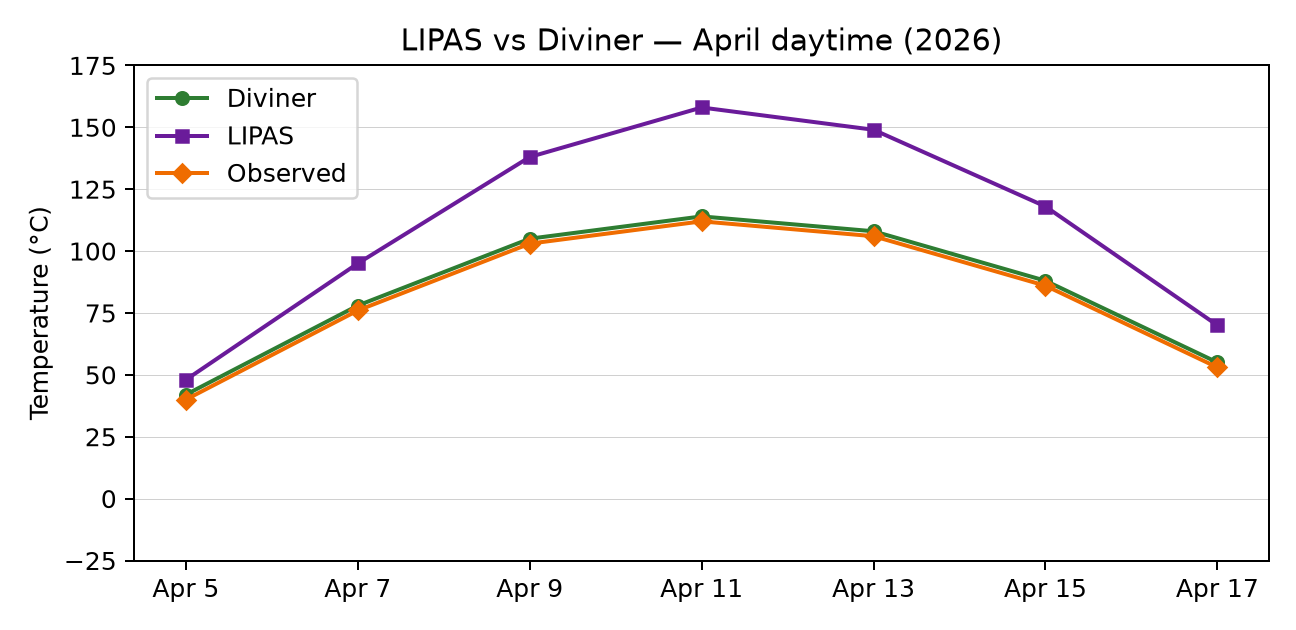
\includegraphics[width=\linewidth]{figures/fig_lipas_vs_diviner.png}
\caption{Daytime temperature at $0^{\circ}$N, $0^{\circ}$E, 5 to 19 April 2026. The prototype rises above the Diviner-style estimate near the warmest part of the day.}
\label{fig:diviner}
\end{figure}

Figure 5: Daytime temperature at 0$^\circ$N, 0$^\circ$E, 5 to 19 April 2026. The prototype rises above the Divinerstyle estimate near the warmest part of the day. The prototype overshoots the Divinerstyle estimate near peak heating. fourteen-day studies. Figures 4 and 5 are the April check only; they are not repeated in Windows A and B. \subsection{Qualitative comparison}

LIPAS and six reference systems were scored on the nine criteria in Section 4.2. DONKI monitors events, Diviner and LDEX archive measurements, Apollo PSE is a historical catalog, MEM 3 is a statistical engineering model, and GOES-18 is a real-time monitor used here from Earth orbit. Scores run from None to Very High and are not added up. VH = Very High; H = High; M = Moderate; L = Low; VL = Very Low; N = None. Specialist systems score high where they were built to be strong, and low on fusion and forecasting. LIPAS is scored high where the interface has to carry several hazards at once. The matrix is not a ranking, and it does not say that LIPAS is more accurate than a specialist archive. Table 2: Qualitative comparison of LIPAS with selected agency models and archives. Criteria follow Section 4.2. Labels are not summed. VH = Very High; H = High; M = Moderate; L = Low; VL = Very Low; N = None. This overshoot keeps temperature on the physics path in the

Window A covers 5 to 18 July 2026 at 0$^\circ$N 0$^\circ$E, Apollo 11, and Nobile Rim (42 site-days). Local solar time was mostly night. The same blend and the same references are used at every site. \begin{figure}[t]
\centering
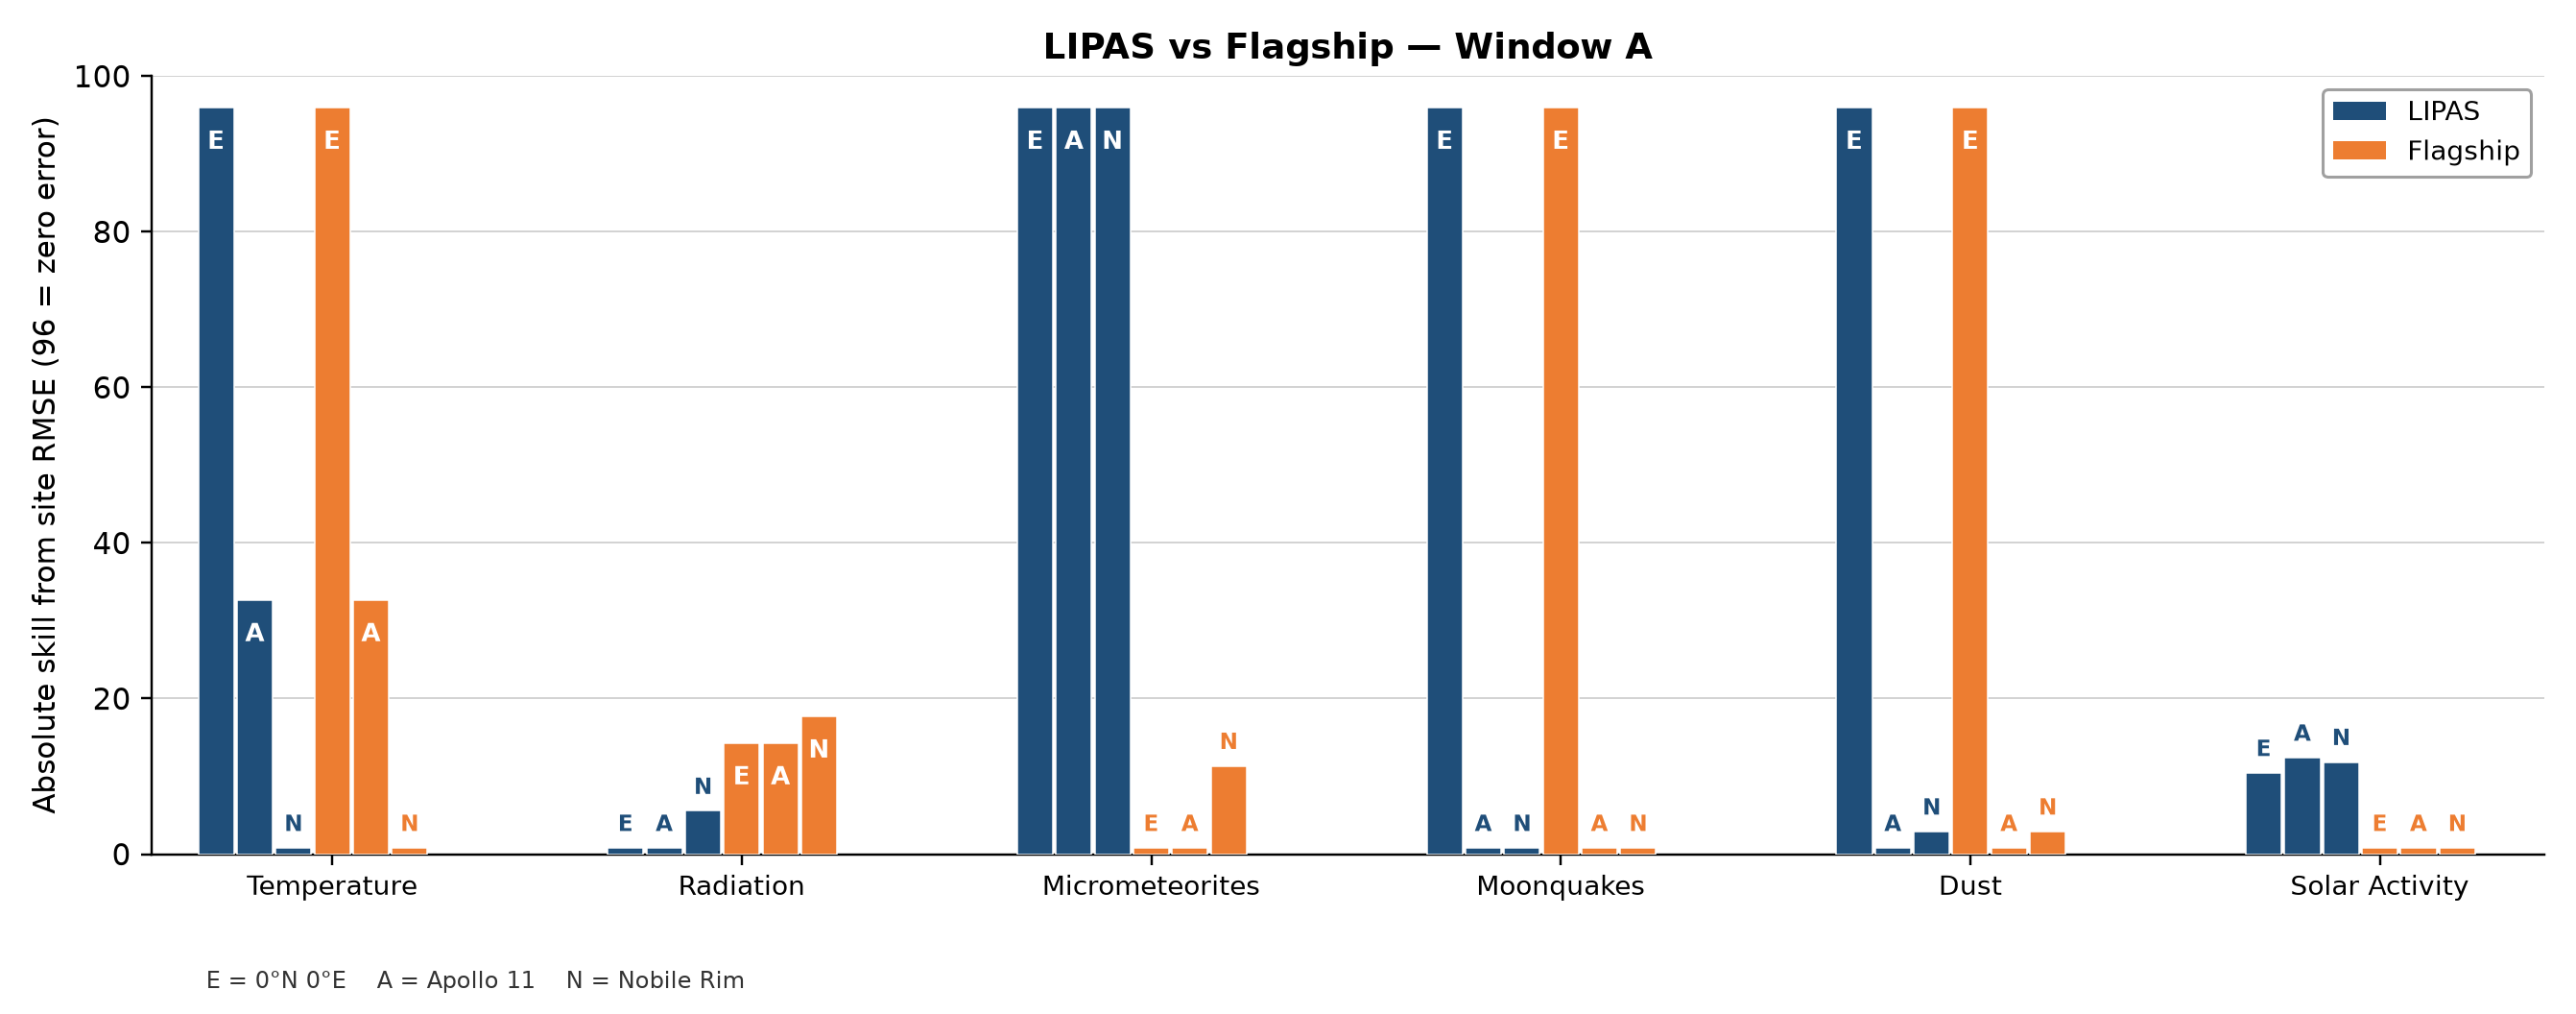
\includegraphics[width=\linewidth]{figures/fig_windowA_skill.png}
\caption{Window A skill from per-site RMSE (5 to 18 July 2026; 42 site-days). E = $0^{\circ}$N $0^{\circ}$E; A = Apollo 11; N = Nobile Rim. Navy is LIPAS; orange is the replica.}
\label{fig:winAskill}
\end{figure}

Figure 6: Window A skill from per-site RMSE (5 to 18 July 2026; 42 site-days). E = 0$^\circ$N 0$^\circ$E; A = Apollo 11; N = Nobile Rim. Navy is LIPAS; orange is the replica. \begin{figure}[t]
\centering
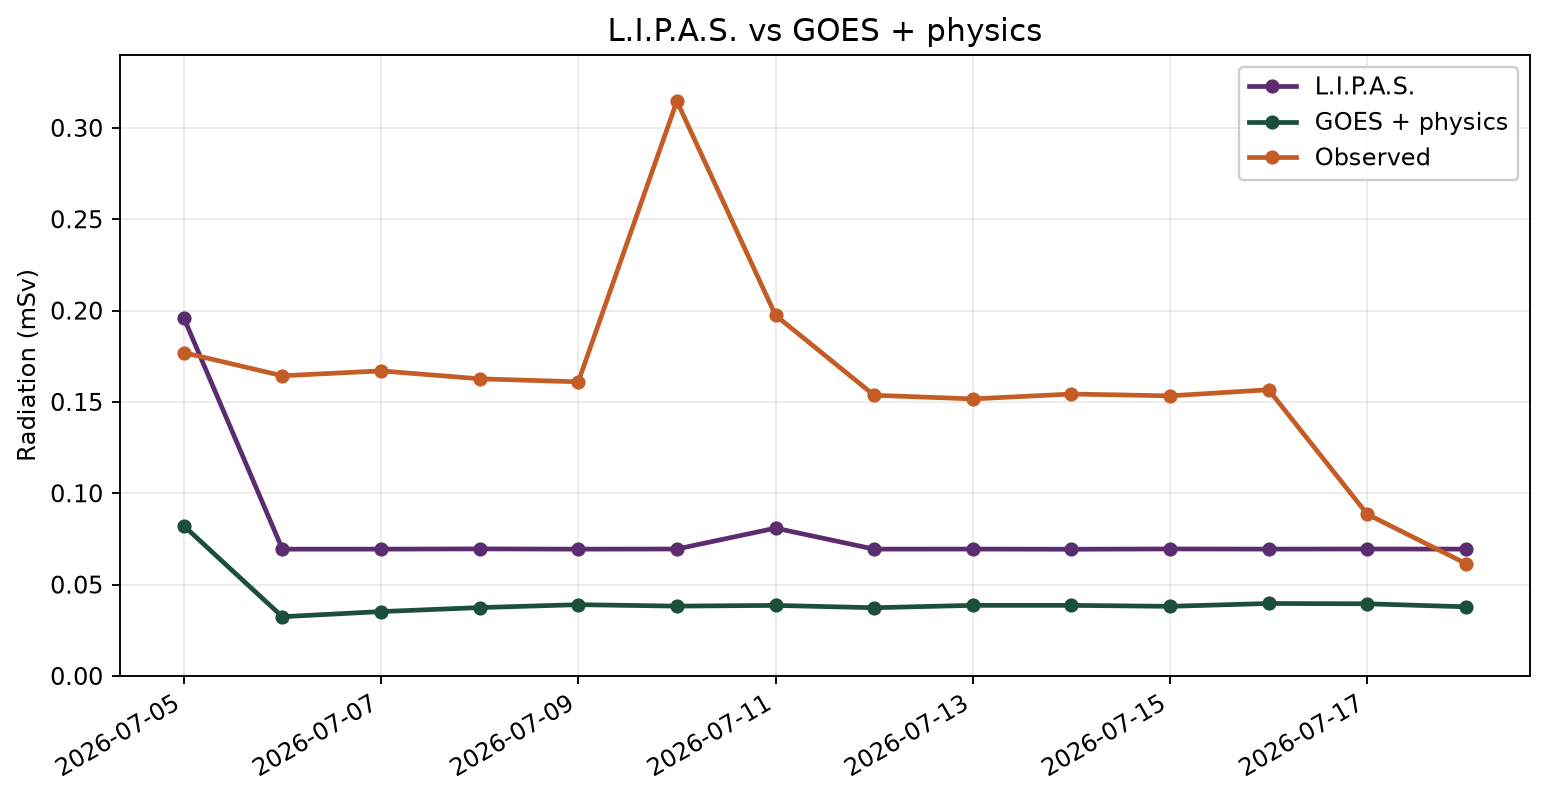
\includegraphics[width=\linewidth]{figures/fig_windowA_radiation.png}
\caption{Window A radiation. LIPAS, the GOES-plus-physics reference, and the evaluation labels.}
\label{fig:winArad}
\end{figure}

Figure 7: Window A radiation. LIPAS, the GOES-plus-physics reference, and the evaluation labels.

\subsection{Fourteenday evaluation}

\subsubsection{Window A, predominantly lunar night}

Solar activity shows a modest gain for the hybrid (RMSE 4.10 versus 4.66). Radiation RMSE stayed higher for the hybrid (0.119 versus 0.102). Temperature, moonquakes, and dust match because they share a physics path. The micrometeorite bars use blend weight zero and are not an independent win. Skill 96 = zero site RMSE, not a percent score. Replica stays closer to the labels than the hybrid here.

Table 3: Window A RMSE, 5 to 18 July 2026, lunar-night dominant, 42 site-days. Hazard Hybrid Replica Outcome Solar activity 4.10 4.66 Hybrid lower by about 12\% Radiation (mSv) 0.119 0.102 Replica lower Temperature ($^\circ$C) 38.2 38.2 Tie, shared physics path Moonquakes / day 1.23 1.23 Tie, shared physics path Micrometeorites 0.0 0.624 Not an independent win Dust (g cm-3) 0.526 0.526 Tie, shared physics path Window B uses the same sites, blend, and metrics on 22 July to 4 August 2026 (42 site-days). About 95 percent of the site-days are on the dayside. For micrometeorites, LIPAS carries a shower-timing term, including the Perseids near 4 August, and the replica uses the seasonal MEM 3 envelope without that term. \begin{figure}[t]
\centering
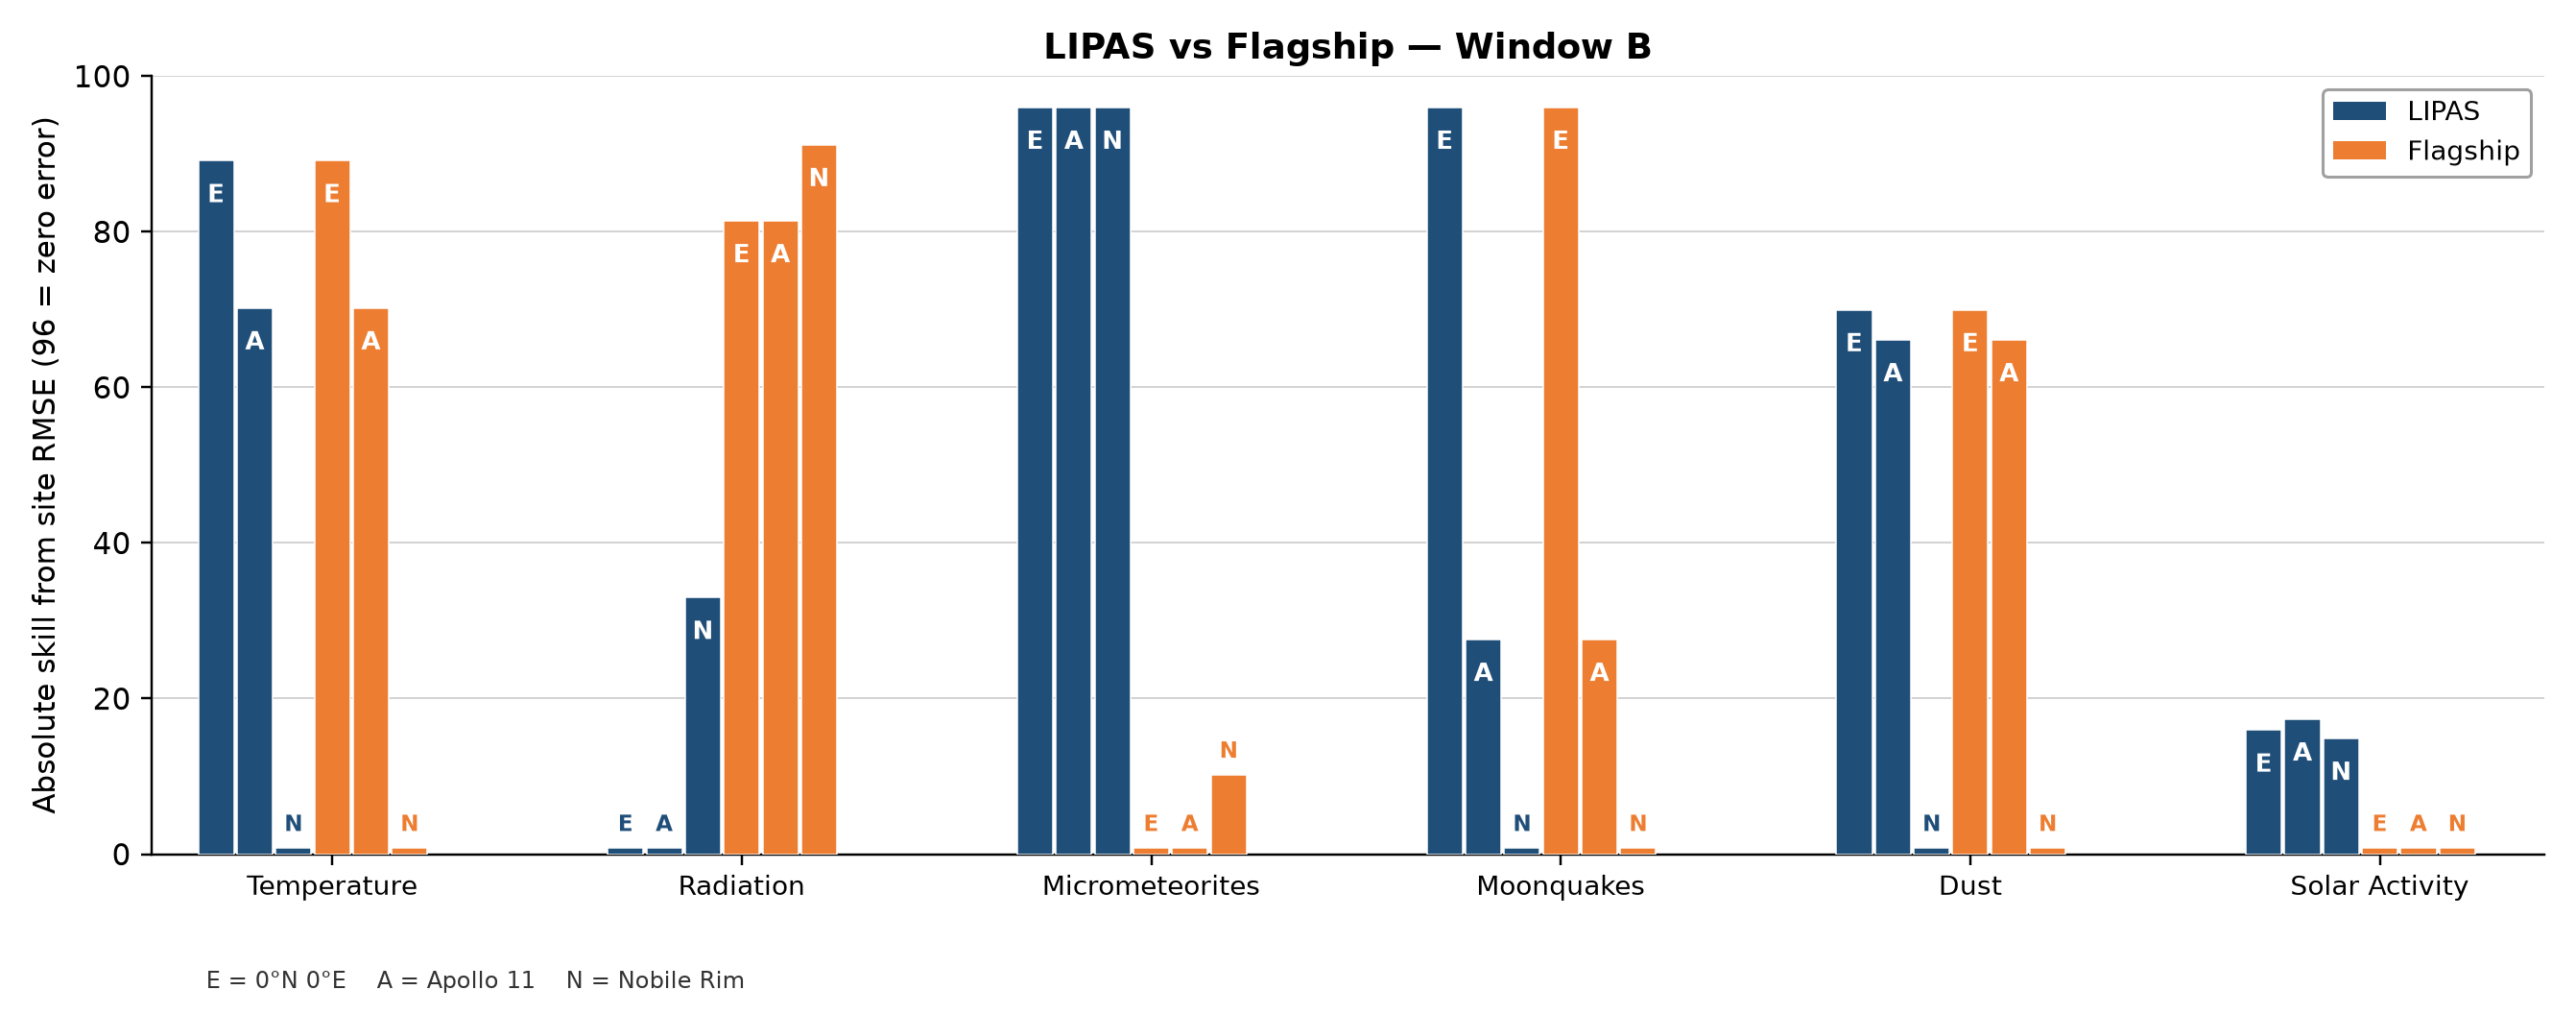
\includegraphics[width=\linewidth]{figures/fig_windowB_skill.png}
\caption{Window B skill from per-site RMSE (22 July to 4 August 2026; 42 site-days). Same site letters and replica as Window A.}
\label{fig:winBskill}
\end{figure}

Figure 8: Window B skill from per-site RMSE (22 July to 4 August 2026; 42 site-days). Same site letters and replica as Window A.

\subsubsection{Window B, predominantly lunar day}

Solar activity is again lower for the hybrid (4.99 versus 5.99). Radiation is not: in this quiet dayside window the replica is

0.00266 and the hybrid is 0.0188. Temperature, moonquakes, and dust remain ties (Table 4).

Table 4: Window B RMSE, 22 July to 4 August 2026, lunar-day dominant, 42 site-days. Hazard Hybrid Replica Outcome Solar activity 4.99 5.99 Hybrid lower by about 17\% Radiation (mSv) 0.0188 0.00266 Replica lower (quiet dayside) Temperature ($^\circ$C) 25.5 25.5 Tie, shared physics path Moonquakes / day 0.695 0.695 Tie, shared physics path Micrometeorites 0.0 0.701 Shower term only Dust (g cm-3) 0.169 0.169 Tie, shared physics path \begin{figure}[t]
\centering
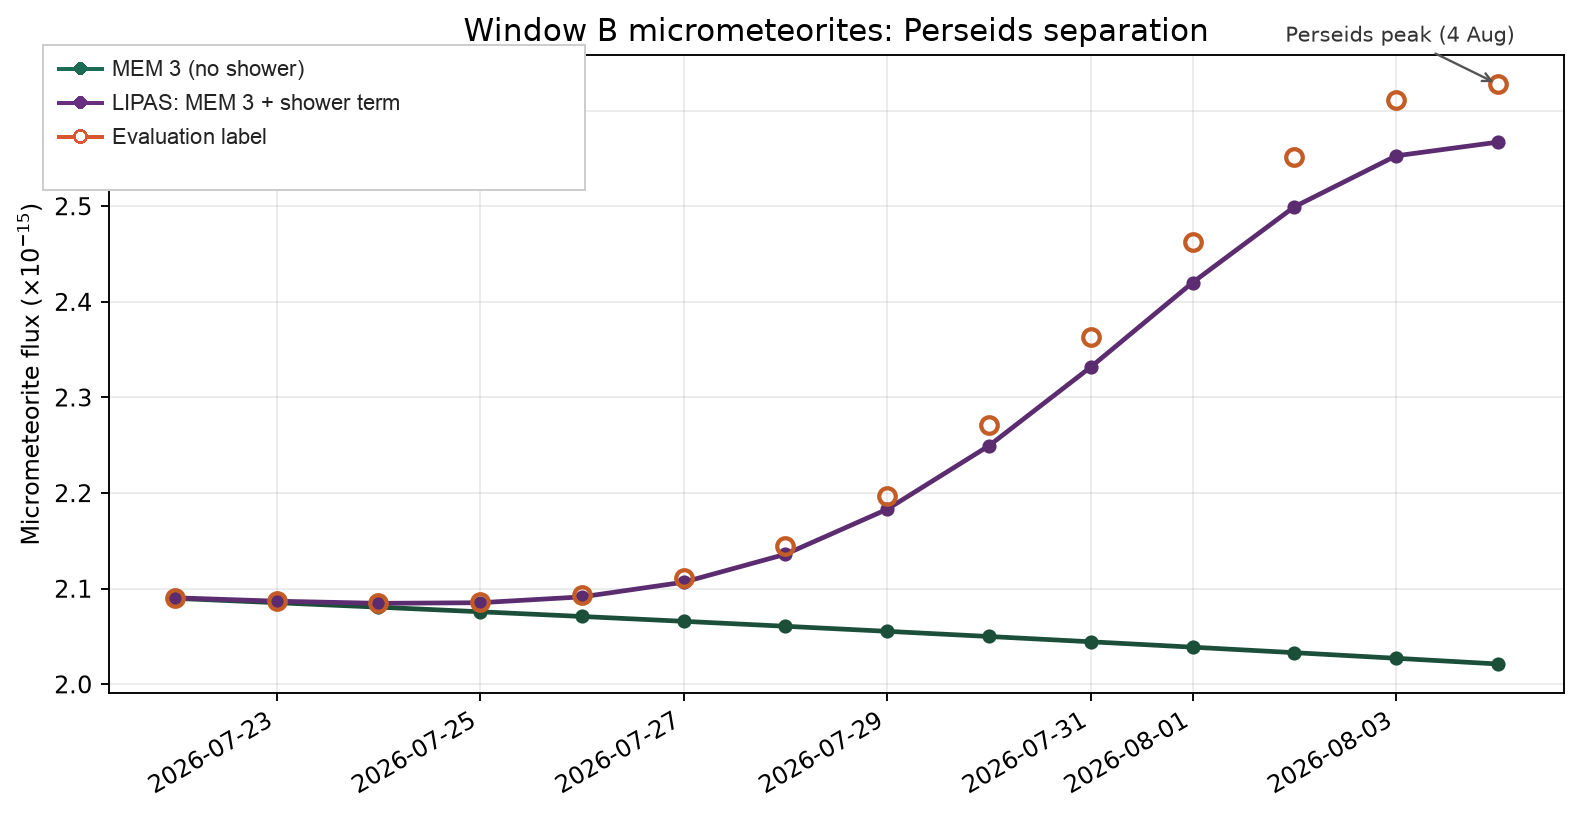
\includegraphics[width=\linewidth]{figures/fig_windowB_meteors.png}
\caption{Window B study-site mean micrometeorite flux. LIPAS includes the shower-timing term. The comparison curve is MEM 3 without it.}
\label{fig:meteors}
\end{figure}

Figure 9: Window B studysite mean micrometeorite flux. LIPAS includes the shower-timing term. The comparison curve is MEM 3 without it. The label is the evaluation series, not a surface impact measurement.

\subsection{Operational mission simulation}

A radiation-focused EVA at the Apollo 11 site was simulated over 7 h 37 min, the duration of the second Apollo 17 EVA, to compare LIPAS warning times with those of separate public products. The same storm was injected on every path: a precursor at T+40, rising Kp and southward IMF Bz at T+55, and a GOESlike proton surge at T+70. Every path used the same thresholds, 0.095 mSv h-1 for caution and 0.15 mSv h-1 for no-go. The GOES-only path used proton flux alone, and the combined NASA path took the earlier of the proton warning and the geomagnetic or solardriver warning. \begin{figure}[t]
\centering
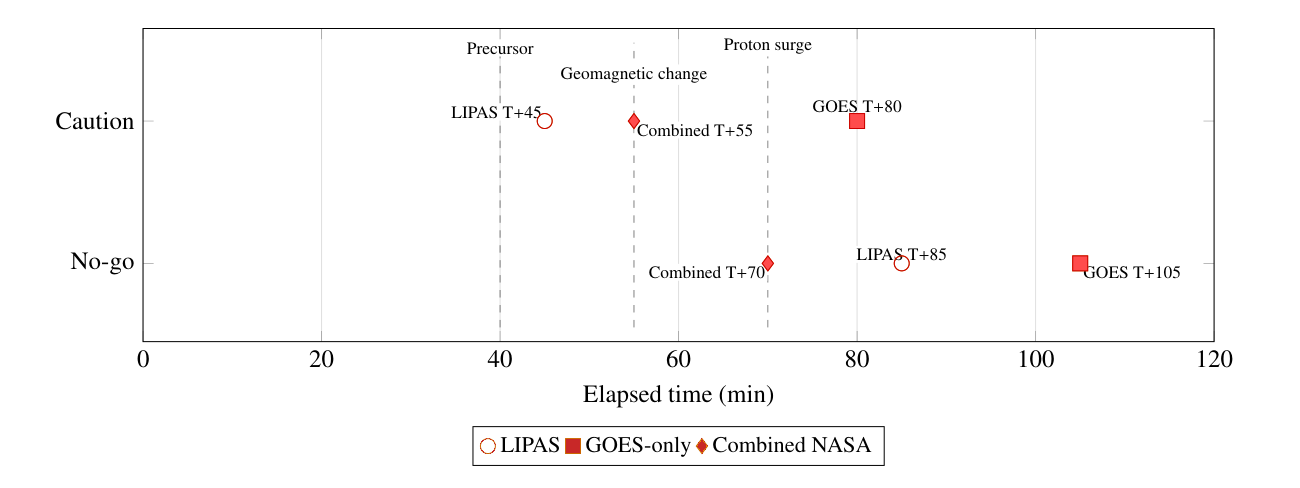
\includegraphics[width=\linewidth]{figures/fig_mission_timeline.png}
\caption{Mission-simulation decision timeline. Open circles are LIPAS, squares are GOES-only, and diamonds are the combined NASA path.}
\label{fig:mission}
\end{figure}

Figure 10: Missionsimulation decision timeline. Open circles are LIPAS, squares are GOES-only, and diamonds are the combined NASA path. Dashed lines mark the precursor, geomagnetic change, and proton surge. LIPAS issued caution at T+45 and no-go at T+85. GOES alone reached caution at T+80 and no-go at T+105, and the combined path reached caution at T+55 and no-go at T+70. The earlier LIPAS caution came from upstream solar and geomagnetic drivers, not from an event the proton product could not see. The exercise is radiation-focused. It does not show that LIPAS is safer on every hazard, and it does not replace an operator or flight-certified products.

Table 5: Radiation-channel sensitivity results from input ablation. Changes are full-model RMSE minus configuration RMSE. Configuration RMSE Full minus case Relative change Full model 0.1020 0.0000 0.0\% Set solar to mean 0.1050 -0.0029 -2.9\% Set radiation to mean 0.1029 -0.0009 -0.9\% Set temperature to mean 0.1020 ~0 ~0\% Set moonquakes to mean 0.1020 ~0 ~0\% Set micrometeorites to mean 0.1020 ~0 ~0\% Set dust to mean 0.1020 ~0 ~0\% Set solar and radiation to mean 0.1068 -0.0048 -4.7\% Table 6: Solar-activity sensitivity results from input ablation. Changes are full-model RMSE minus configuration RMSE. Configuration RMSE Full minus case Relative change Full model 3.899 0.000 0.0\% Set micrometeorites to mean 3.984 -0.085 -2.2\% Set radiation to mean 3.933 -0.034 -0.9\% Set moonquakes to mean 3.931 -0.032 -0.8\% Set temperature to mean 3.916 -0.018 -0.5\% Set dust to mean 3.909 -0.011 -0.3\% Set solar to mean 3.290 +0.608 +15.6\% (lower RMSE) Set moonquakes and dust to mean 3.960 -0.061 -1.6\%

\subsection{Input ablation}

The ablation study keeps the locked model fixed and uses a relatively quiet portion of the Window A data. One input at a time, and two input pairs, are replaced with their Window A averages; the model is not retrained. Tables 5 and 6 report the resulting RMSE values. In the full-minus-case column, a negative value means that the altered configuration had a higher error than the full model. On the radiation channel, replacing the live solar input with its Window A average raised RMSE from 0.1020 to 0.1050 (about 2.9\%). Replacing any other single input left radiation RMSE essentially unchanged, and replacing solar and radiation together raised it further, to

0.1068 (about 4.7\%).

On the solar channel, the same replacement lowered RMSE from 3.899 to 3.290 (about 15.6\%). This is a sensitivity result for a quiet window and does not show that live solar data are generally harmful; Section 6 discusses possible explanations. The other single and paired replacements changed solar RMSE by 2.2\% or less.

\section{Discussion}

The studies reported in Section 5 show that the usefulness of machine learning, physics-based modelling and data integration in LIPAS depends on the hazard being forecast and on the purpose for which the output is used. This section interprets those results, sets out what they do and do not show, and identifies the limitations that bound the answers to the research questions given in Section 8. Combining physics and machine learning is not itself new (Karpatne et al., 2017; Willard et al., 2022; Camporeale, 2019). Theoryguided and physicsinformed approaches have already been applied across environmental and space-weather problems. The contribution of LIPAS is narrower: the application of hazard-specific weighting, uncertainty-aware blending and cross-hazard inputs within a single lunar forecasting and decision-support system. In LIPAS the Python physics\_estimate function supplies a physically grounded value for each hazard, the learned correction from the LSTM trunk is blended with it through Eqs. (2) and (3), and public heliophysics data enter as inputs to both paths rather than as a third modelling method. The results provide preliminary support for this design, while also showing that the architecture should not be treated as a replacement for specialised scientific models or as a fully validated operational forecasting system. The development record is important for interpreting the final architecture, and it must be read separately from the quantitative evidence. The April diagnostics used the browser prototype, not the locked hybrid model, and compared it with weakly replicated baselines at a single daytime site. The prototype scored higher than those weak replicas on five of the six hazards, but that comparison was designed to expose failure modes rather than to measure skill, and its scores are not pooled with the locked-model results. Its actionable finding was the temperature overshoot against the Divinerstyle dayside relation near peak heating, together with run-to-run variation in physically constrained channels. These observations motivated the migration to a server-assisted backend and the decision to keep temperature, moonquakes, micrometeorites and dust on the physics path. Every quantitative claim in Windows A and B, the mission simulation and the ablation therefore rests on the locked production model from the second training run. The ties on temperature, moonquakes and dust follow directly from how the system and the evaluation were constructed. The locked blend weights are [0.4, 0.05, 0, 0, 0, 0] for solar activity, radiation, temperature, moonquakes, micrometeorites and dust. With a weight of zero, the hybrid output for those channels is the physics\_estimate output. The replicated public baselines and the evaluation labels for the same channels were built from the same public archives and formulations. Identical RMSE values (38.2, 1.23 and 0.526 in Window A; 25.5, 0.695 and 0.169 in Window B) are therefore expected by construction. They show that the hybrid did not introduce unnecessary neural corrections where physics already provides a strong foundation, but they are not evidence of skill over the references and they are not independent validation. More generally, much of the data and many of the approaches used to build the comparison targets overlap with those used to build LIPAS itself. Where that overlap is large, agreement between LIPAS and its references partly measures internal consistency rather than predictive accuracy. This is also why the uncertainty-guided weighting matters. LIPAS does not simply average a machine-learning prediction with a physics estimate. Within each channel's locked base weight, Eq. (3) reduces the learned contribution when the Monte Carlo dropout spread widens, shifting the forecast toward the physics path when the network is less certain. The purpose of the architecture was not to force machine learning into every channel, but to allow different sources of information to carry different levels of influence. Solar activity provides the clearest evidence that the learned correction and heliophysics inputs can add predictive information. It is the channel with the largest learned weight (0.4), and the hybrid RMSE was lower than the replica in both windows: 4.10 versus 4.66 in the predominantly nightside Window A, and 4.99 versus 5.99 in the predominantly dayside Window B. Because the gain appears in both lunar regimes rather than in only one, it is less likely to be an artefact of a single window. It remains modest, however, and it is based on two fourteen-day windows at three sites (42 site-days each). Radiation did not improve. The replica had lower RMSE in Window A (0.102 versus 0.119 for the hybrid) and in the quiet dayside Window B (0.00266 versus 0.0188). In Window B both errors are small in absolute terms, but the replica is still clearly ahead. The learned weight on radiation is small (0.05), and the present studies do not isolate whether the gap arises from the learned correction, from the radiation physics path and its inputs, or from the construction of the evaluation labels against which both paths were scored. The radiation channel should therefore be read as a current weakness of LIPAS rather than as a demonstrated strength. The micrometeorite results need equally careful reading. The channel has a blend weight of zero, so the hybrid output is the physics path, which combines the MEM 3 export with AMSbased shower modulation. The evaluation series used for scoring carries the same shower term. The hybrid RMSE of 0.0 in both windows is therefore circular and is not an independent win; the replica errors (0.624 in Window A and 0.701 in Window B) measure the absence of the shower term rather than a deficiency of the MEM 3 framework. The separation between the two curves as the Perseids approached in Window B illustrates the effect of adding shower timing to a seasonal background model. It does not demonstrate superiority over the complete NASA micrometeorite modelling framework, and it is not validated against measured lunar impact rates. The mission simulation shows why predictive performance and operational usefulness are not the same thing. In the radiation-focused EVA scenario, LIPAS issued caution at T+45, five minutes after the injected precursor at T+40 and 25 minutes before the proton surge at T+70, and reached no-go at T+85. The GOES-only path reached caution at T+80 and no-go at T+105, while the combined NASA path reached caution at T+55 and the earlier hard no-go at T+70. The earlier LIPAS caution came from upstream solar and geomagnetic drivers, not from an event that the proton product could not see. The result should not be interpreted as LIPAS detecting a storm that NASA could not detect. Instead, it shows that different pathways produce different warning times depending on which signals they monitor and how those signals are mapped to thresholds. The scenario used a single injected storm, predefined caution and no-go thresholds, and one hazard. It did not measure usability with mission personnel, it does not show that LIPAS is safer on every hazard, and it is not a proof of operational safety. A unified system can also concentrate risk if its data feeds or service fail, which a set of independent products partly avoids. replica

The ablation study provides evidence of cross-hazard sensitivity inside the locked model, but not of causation. It used a relatively quiet portion of Window A and replaced one input at a time with its window mean, without retraining. On the radiation channel, replacing the solar input raised RMSE from 0.1020 to 0.1050 (about 2.9\%), and replacing solar and radiation together raised it to 0.1068, while other single replacements left it essentially unchanged. On the solar channel, the same replacement lowered RMSE from 3.899 to 3.290, while the other replacements changed solar RMSE by about 2\% or less (for example, replacing radiation changed it by 0.034, or 0.9\%). Several explanations are possible for the solar result: shortterm variation in the live solar input may not match the smoother evaluation labels, the current weighting may give that input too much influence under quiet conditions, or the construction of the labels may favour a smoother representation of the underlying signal. The ablation measures how far the output moves when one input is held at its average; it does not show that one hazard causes another, and the lower solar error does not show that live solar data are generally harmful. Looking across the full set of results, different hazards benefit from different forms of information. Temperature, moonquakes and dust remained on their physics paths, and their agreement with the references reflects that shared construction. Solar activity showed modest evidence that the learned correction and cross-hazard inputs can add predictive value. Radiation did not, despite its dependence on solar context in the ablation. Micrometeorite behaviour was determined by explicit shower timing rather than by machine learning. LIPAS therefore does not behave as six identical machine-learning models; it acts as a framework that assigns different levels of influence to different sources of information depending on the hazard. Several limitations affect the strength of these conclusions. First, continuous colocated lunarsurface measurements do not exist for all six hazards, so quantitative targets are evaluation labels constructed from public observations, physical formulations, historical catalogs and proxies. The results describe comparative behaviour within this evaluation framework, not accuracy against complete lunarsurface truth. Second, except for the available MEM 3 engineeringmodel export, the comparisons are replicas: author-built reconstructions of publicly documented methods and data, not executions of agency operational software. Their value is methodological comparability under shared inputs, dates and locations, and they should not be read as runs of the agencies' own systems. Third, the qualitative comparison in Section 5.2 is a criteria matrix, not a ranking, and it does not say that LIPAS is more accurate than any specialist archive or model. Fourth, the quantitative evidence covers two fourteen-day windows, three sites and one locked model, and the radiation conditions in both windows were relatively quiet. The strongest conclusion is therefore not that LIPAS replaces specialised NASA or NOAA models. Its value lies in providing a common forecasting and decision-support layer in which established physics, public heliophysics inputs, cross-hazard relationships and uncertainty estimates can be considered together. The results support this concept as a promising direction, while showing that substantial validation is still required before operational use.

\section{Future work}

LIPAS already provides a multi-hazard decision-support system for lunar operations, but further work is needed before it can be considered a trusted operational forecasting tool. The fourteen-day windows, mission simulation and ablation study have clarified where that work should focus. Rather than repeating the evaluations already completed, future work should build directly on their findings.

\subsection{Radiation across activity regimes}

The radiation channel is the highest priority, because the locked hybrid did not outperform the replicated public baseline in either window. Future work should evaluate radiation across a wider range of solar activity, including disturbed and storm periods, and should identify which component of the radiation path accounts for the current gap. Potential improvements include denser OMNI, DONKI and SWPC sampling, improved treatment of protonflux events, calibrated uncertainty estimates for radiation alerts, and validation against additional historical space-weather events. Differences between LIPAS and the combined NASA warning path should be examined transparently rather than resolved by retrospective threshold tuning.

\subsection{Solar input behaviour}

The solar ablation result deserves closer investigation. Repeating the ablation under stronger solar activity, and with retrained rather than mean-substituted configurations, would show when the live solar input provides the greatest benefit and whether its influence under quiet conditions should be reduced. The modest solar gain should also be tested over longer periods and additional sites.

\subsection{Physicstied channels and independent labels}

Temperature, moonquakes, dust and micrometeorites should remain physics-led, but their evaluation needs targets that are independent of the physics path. Future work should strengthen meteorshower timing and MEM 3 integration, and should score micrometeorites against observations that do not already contain the LIPAS shower term, so that the channel can be assessed rather than only described.

\subsection{Validation with measured data}

As data become available from Artemis missions, lunar landers, rovers and orbital instruments, evaluation labels should be replaced with direct measurements wherever possible. Where measurements are not yet available, estimated labels should continue to be identified clearly. Collaboration with NASA, NOAA, ESA, JAXA and university research groups would strengthen validation through access to additional datasets, operational expertise and missionrelevant performance criteria.

\subsection{Operational development}

Future development of the LIPAS interface and mission planner should improve uncertainty visualisation, mission-specific alert thresholds and reports aligned with existing operational checklists. Mission simulations should extend beyond a single radiation storm to multi-hazard scenarios, should test behaviour when data feeds fail, and should measure usability with mission personnel. Interface improvements are valuable only if they communicate the underlying scientific results accurately and transparently. replica

\subsection{Extending the framework beyond the lunar surface}

Because much of the system already relies on heliophysics data, extending the framework to cislunar space and Earth orbit is a logical next step, with Mars as a longerterm possibility. These environments offer substantially more observational data than the lunar surface, allowing more rigorous validation of the hybrid method. The multi-hazard architecture and channelspecific weighting could be reused without a complete redesign. The immediate priorities are therefore to diagnose and improve the radiation channel, explain the solar ablation behaviour, and obtain independent evaluation labels for the physics-tied channels. Over the medium term, measured data and collaboration with space agencies should improve confidence in the system. Throughout its development, LIPAS should remain a consultative decision-support platform designed for incomplete observations, used alongside NASA and NOAA products rather than as a replacement for specialised scientific models or flightqualified systems.

\section{Conclusion}

This research examined whether machine learning can be integrated into a unified, physics-based lunar forecasting system while retaining the physical foundations of established environmental models. Regarding the first research question, a hybrid lunarforecasting system can be developed by combining machine-learning and physics-based approaches. The development process showed that a hazard-specific blend was more appropriate than applying machine learning uniformly: the prototype diagnostics exposed instability in physically constrained channels, which led to a locked hybrid model in which solar activity and radiation carry learned weights while temperature, moonquakes, micrometeorites and dust remain on the physics path. The second research question asked whether integrating multiple hazards and data sources into one decision-support system can improve operational usability. The radiation-focused mission simulation answered it partially: LIPAS issued caution earlier than the GOES-only path because it drew on upstream solar and geomagnetic drivers, but the combined NASA path reached the hard no-go first, and the study did not establish that LIPAS is safer than existing approaches. The third research question asked whether the locked hybrid improves prediction performance relative to replicated public baselines and physicsonly references. The answer is mixed. Solar activity improved modestly in both windows; radiation did not; temperature, moonquakes and dust tied because they share a physics construction with their references; and the micrometeorite contrast, under blend weight zero, describes the shower term rather than independent skill. The principal contribution of LIPAS is therefore not the replacement of existing lunar models but their integration into a single forecasting and decision-support framework. The studies show both where a constrained hybrid architecture can add predictive value and where it does not yet do so, and they define the validation that must follow before LIPAS can support lunar operations alongside NASA and NOAA products.

\section*{Acknowledgements}

The author thanks Benjamin Irani-Fey for coding support during the NASA Space Apps Challenge. The author also thanks NASA, NOAA, and other space agencies and research organizations for the public lunarmission data and space-weather archives that made the project possible, and thanks Polygence research mentor Kyle Kennedy for support in redesigning and reevaluating the studies, methods, and conclusions. CRediT author statement Luka Takki: Conceptualization, Methodology, Software, Validation, Formal analysis, Investigation, Data curation, Visualization, Writing --- original draft, and Writing --- review and editing. This research received no specific grant from funding agencies in the public, commercial, or not-for-profit sectors. Declaration of competing interest The author declares that there are no known competing financial interests or personal relationships that could have appeared to influence the work reported in this paper. Data and code availability Public sources are listed in the references; numerical tables accompany the paper. Dashboard: \url{https://lipas.netlify.app}. Code: \url{https://github.com/Luka-bot-afk/LIPAS} (numerical tables in the papers/appendix\_numerical\_tables folder).

\section*{Declaration of generative AI and AI-assisted technologies in the manuscript preparation process}

During the preparation of this work, the author used Cursor and Google Gemini to review, and to help modify, selected parts of the code and the manuscript. These tools did not write the paper. The author checked every suggested change, made the final edits, and takes full responsibility for the content of the published article. Their role was limited to review and selective modification of existing material; they were not used to draft or author the manuscript. 

\section*{References}

American Meteor Society, 2026. Meteor shower calendar. URL: \url{https://www.amsmeteors.org/meteor-showers/meteor-shower-calendar}. Camporeale, E., 2019. The challenge of machine learning in space weather: Nowcasting and forecasting. Space Weather 17, 1166-1207. doi:10.1029/2018SW002061. Cesium GS, 2026. Cesiumjs 3d geospatial virtual globe engine. URL: \url{https://cesium.com}. Chart.js Contributors, 2026. Chart.js open-source canvas graphing toolset. URL: \url{https://www.chartjs.org}. Chollet, F., et al., 2015. Keras. URL: \url{https://keras.io/}. Colwell, J.E., Batiste, S., Horanyi, M., Robertson, S., Sture, S.,

2007. Lunar surface: Dust dynamics and regolith mechanics.

Reviews of Geophysics 45, RG2006. doi:10.1029/2005RG 000184. Cucinotta, F.A., Hu, S., Schwadron, N.A., Kozarev, K., Townsend, L.W., Kim, M.H.Y., 2010. Space radiation risk limits and earth-moon-mars environmental models. Space Weather 8, S00E09. doi:10.1029/2010SW000572. Google TensorFlow Team, 2026. Tensorflow machine learning and deep learning ecosystem. URL: \url{https://www.tensorflow.org}. Hassler, D.M., et al., 2014. Mars' surface radiation environment measured with the mars science laboratory's curiosity rover. Science 343, 1244797. doi:10.1126/science.1244797. Hayne, P.O., Williams, J.P., Bandfield, J.L., Vasavada, A.R., Greenhagen, B.T., Siegler, M.A., Paige, D.A., Tyler, G.L.,

2017. Global regolith thermophysical properties of the moon

from the lunar reconnaissance orbiter diviner radiometer. Journal of Geophysical Research: Planets 122, 2371-2400. doi:10.1002/2017JE005387. Hochreiter, S., Schmidhuber, J., 1997. Long short-term memory. Neural Computation 9, 1735-1780. doi:10.1162/neco.199 7.9.8.1735. Horanyi, M., Szalay, J.R., Kempf, S., Schmidt, J., Grun, E., Srama, R., Sternovsky, Z., 2015. A permanent, asymmetric dust cloud around the moon. Nature 522, 324-326. doi:10.1 038/nature14479. International Meteor Organization, 2026. Meteor shower calendar resources. URL: \url{https://www.imo.net/resources/calendar}. Karpatne, A., et al., 2017. Theory-guided data science: A new paradigm for scientific discovery from data. IEEE Transactions on Knowledge and Data Engineering 29, 2318-2331. doi:10.1109/TKDE.2017.2720168. Kawamura, T., Tanaka, S., Saito, Y., Horleston, A.C., Charalambous, C., Lognonne, P., Banerdt, W.B., Team, A.S., 2017. Re-analysis of apollo seismic data and implications for deep moonquakes. Journal of Geophysical Research: Planets 122, 114-132. doi:10.1002/2016JE005230. King, J.H., Papitashvili, N.E., 2005. Solar wind spatial scales in and comparisons of hourly wind and ace plasma and magnetic field data. Journal of Geophysical Research 110, A02104. doi:10.1029/2004JA010649. Lammlein, D.R., 1977. Lunar seismicity and tectonics. Physics of the Earth and Planetary Interiors 14, 224-273. Langseth, M.G., Keihm, S.J., Peters, K., 1972. Revised lunar heat-flow values, in: Proceedings of the Third Lunar Science Conference, MIT Press. pp. 3143-3171. Minow, J.I., et al., 2020. Space Weather Architecture Options to Support Human and Robotic Deep Space Exploration. Technical Report NASA/TM-20205000837. NASA. URL: \url{https://ntrs.nasa.gov/citations/20205000837}. Moorhead, A.V., Koehler, H.M., Cooke, W.J., 2020. NASA Meteoroid Engineering Model Release 3 (MEM 3). Technical Report. NASA. URL: \url{https://ntrs.nasa.gov/citations/20200001093}. Nakamura, Y., 2005. Farside deep moonquakes and deep interior of the moon. Journal of Geophysical Research: Planets 110, E01001. doi:10.1029/2004JE002332. NASA, 2020. Nasa's lunar exploration program overview. URL: \url{https://www.nasa.gov/specials/artemis/}. NASA, 2023a. Diviner lunar radiometer experiment data products. URL: \url{https://pds-geosciences.wustl.edu/lro/lro-l-dlre-4-rdr-v1.0/}. NASA, 2023b. Donki api documentation. URL: \url{https://api.nasa.gov/DONKI/}. NASA, 2023c. Lro crater data products. URL: \url{https://pds-geosciences.wustl.edu/missions/lro/crater.htm}. The reported experiments are reproduced in Supplementary Appendices A to D. Code and locked model files: \url{https://github.com/Luka-bot-afk/LIPAS}. Daily tables are in papers/appendix\_numerical\_tables/. 

NASA Goddard Space Flight Center, 2026. Space physics data facility omni database. URL: \url{https://omniweb.gsfc.nasa.gov}. NASA Planetary Data System, 2015. Ladee ldex calibrated data. National Oceanic and Atmospheric Administration, 2023. Space weather prediction center datasets: Goes primary x-ray flux, integral protons, and planetary k-index. URL: \url{https://services.swpc.noaa.gov/}. Nunn, C., et al., 2020. Lunar seismology: A data and instrumentation review. Space Science Reviews 216, 89. doi:10.1007/s11214-020-00709-3. Onodera, K., 2024. Reanalysis of apollo seismic data reveals 22,000 previously undetected moonquakes. Journal of Geophysical Research: Planets 129, e2023JE008153. doi:10.1029/2023JE008153. Paige, D.A., et al., 2010. The lunar reconnaissance orbiter diviner lunar radiometer experiment. Space Science Reviews 150, 125-160. doi:10.1007/s11214-009-9529-2. Schwadron, N.A., et al., 2014. Does the worsening galactic cosmic radiation environment observed by crater preclude future manned deep-space exploration? Space Weather 12, 622-632. doi:10.1002/2014SW001084. Spence, H.E., et al., 2010. Crater: The cosmic ray telescope for the effects of radiation experiment on the lunar reconnaissance orbiter mission. Space Science Reviews 150, 243-284. doi:10 .1007/s11214-009-9584-8. Stubbs, T.J., Vondrak, R.R., Farrell, W.M., 2006. A dynamic fountain model for lunar dust. Advances in Space Research 37, 59-66. doi:10.1016/j.asr.2005.04.005. Szalay, J.R., Horanyi, M., 2015. Annual variation and synodic modulation of the sporadic meteoroid flux to the moon. Geophysical Research Letters 42, 10580-10584. doi:10.1002/ 2015GL066898. Vasavada, A.R., Paige, D.A., Wood, S.E., 1999. Near-surface temperatures on mercury and the moon and the stability of polar ice deposits. Icarus 141, 179-193. doi:10.1006/icar .1999.6175. Willard, J., Jia, X., Xu, S., Steinbach, M., Kumar, V., 2022. Integrating scientific knowledge with machine learning for engineering and environmental systems. ACM Computing Surveys 55, 1-37. doi:10.1145/3514228. Williams, J.P., Paige, D.A., Greenhagen, B.T., Sefton-Nash, E., 2017. The global surface temperatures of the moon as measured by the diviner lunar radiometer experiment. Icarus . Zeitlin, C., et al., 2013. Measurements of energetic particle radiation in transit to mars on the mars science laboratory. Science 340, 1080-1084. doi:10.1126/science.1235989.

\appendix
\section{Numerical tables}

The short RMSE tables for Windows A and B are in reported\_window\_rmse.md. The daily rows are in the numerical PDF. If the preview is blank, the Download option opens the file. April rows start after the cover page. Window A daily rows start at the fourteen-day lunar-night heading. Window B daily rows start at the first table dated 22 July. \url{https://github.com/Luka-bot-afk/LIPAS/blob/main/papers/appendix_numerical_tables/reported_window_rmse.md} \url{https://github.com/Luka-bot-afk/LIPAS/blob/main/papers/appendix_numerical_tables/LIPAS_appendix_numerical_tables_A_B_D_E.pdf} The model folder saved\_model is not in the public repository. The files above can be opened without that folder. A fresh copy of the repository can run the scripts only after that folder is on your machine and left unchanged.

\section{Qualitative comparison framework}

DONKI, Diviner, LDEX, Apollo PSE, MEM 3, GOES-18, and LIPAS are scored on the nine criteria. The labels run from None to Very High. Labels are not converted into numbers or summed. Scores can be compared with Table 2. The file also lists the documents used for each score. \url{https://github.com/Luka-bot-afk/LIPAS/blob/main/papers/appendix_numerical_tables/LIPAS_qualitative_comparison_framework.md} The nine criteria Hazard coverage, fusion across hazards, forecast lead, spatial detail, real-time use, robustness, validation, usability, and openness. Documents used NASA DONKI API documentation, \url{https://api.nasa.gov/DONKI/} NOAA SWPC data services, \url{https://services.swpc.noaa.gov/} Paige et al. (2010), Space Science Reviews, Diviner. Williams et al. (2017), Icarus, Diviner global temperatures. Horanyi et al. (2015), Nature, lunar dust and LDEX. Nakamura (2005), Journal of Geophysical Research, deep moonquakes. Nunn et al. (2020), Space Science Reviews, lunar seismology. Moorhead et al. (2020), NASA MEM 3 technical report. Spence et al. (2010) and Schwadron et al. (2014), CRaTER. King and Papitashvili (2005), OMNI solarwind scales.

\section{How the numbers are compared}

Sites and windows Sites are 0$^\circ$N 0$^\circ$E (E), Apollo 11 (A), and Nobile Rim (N). Window A is 5 to 18 July 2026 and is mostly lunar night (42 site-days). Window B is 22 July to 4 August 2026 and is mostly lunar day (42 site-days). The hazards are solar activity, radiation, temperature, moonquakes, micrometeorites, and dust. What 96 means on the skill charts Skill is 96 times the positive part of 1 minus RMSE divided by a hazard scale. The scale for each hazard is the larger site error, so the worst site on that hazard is 0 and a perfect site is 96. Use the same scale for LIPAS and the replica. 96 is not a percent. The blend in this paper is solar 0.4, radiation 0.05, and 0 for temperature, moonquakes, micrometeorites, and dust.

\section{How to rerun each study}

\url{https://github.com/Luka-bot-afk/LIPAS/blob/main/papers/appendix_numerical_tables/REPRODUCTION.md} Qualitative comparison (Table 2) The framework file linked in Appendix B records the scoring rules for the seven systems; labels can be compared with Table 2. April prototype (Figures 4 and 5) The numerical PDF contains the April rows. This daytime run at 0$^\circ$N, 0$^\circ$E is not the fourteen-day result. There is no separate script, and these rows do not belong in Table 3 or Table 4. Window A (Table 3, Figure 6) python scripts/run\_14day\_flagship\_study.py start 20260705 end 20260718 windowlabel A outdir logs/study\_14day\_window\_A\_night modeldir saved\_model csv data/ingested\_extended/extended\_training\_window\_B\_ready.csv. See logs/study\_14day\_window\_A\_night/summary.json. Solar RMSE should be about 4.10 versus 4.66. Radiation should be about 0.119 versus 0.102. Window B (Table 4, Figure 8) The same script, with start 20260722, end 20260804, and window label B. Solar RMSE should be about 4.99 versus 5.99. Radiation should be about 0.0188 versus 0.00266. Mission simulation (Figure 10) python scripts/run\_mission\_sim\_radiation\_eva.py outdir logs/study\_mission\_sim\_radiation\_eva. LIPAS caution is at T+45 and no-go is at T+85. Ablation (Tables 5 and 6) python scripts/run\_hazard\_ablation\_study.py outdir logs/study\_ablation\_window\_A. The model is not retrained. Replacing the live solar input with its Window A average raises radiation RMSE from 0.1020 to 0.1050 and lowers solar RMSE from 3.899 to 3.290.
